%------------------------------------------------------%
%------------------------------------------------------%
%    Modelo de Projeto de TCC - TADS - PI 1 ( IFMS-NA) % 
% NÃO ALTERE OU APAGUE ESSAS INFORMAÇÕES
% ELAS SÃO A CONFIGURAÇÃO DO SEU ARQUIVO.
%-------------------------------------------------------
%-------------------------------------------------------


\documentclass[
	12pt,				% tamanho da fonte
	openright,			% capítulos começam em pág ímpar 
	twoside,			% para impressão em verso e anverso. Oposto a oneside
	a4paper,			% tamanho do papel. 
	%normalfigtabnum,
	%pnumromarab,
	% Opções da classe abntex2
	chapter=TITLE,		% títulos de capítulos convertidos em letras maiúsculasa
	%section=TITLE,		% títulos de seções convertidos em letras maiúsculas
	%subsection=TITLE,	% títulos de subseções convertidos em letras maiúsculas
	%subsubsection=TITLE,% títulos de subsubseções convertidos em letras maiúsculas
	% Opções do pacote babel
	english,			% idioma adicional para hifenização
    spanish,			% idioma adicional para hifenização
	brazil,				% o último idioma é o principal do documento
]{abntex2}

% ----------------------------------------------------------------
%                           PACOTES
% ----------------------------------------------------------------

		

\usepackage[utf8]{inputenc}		% O pacote inputenc é usado para que seja possível escrever textos acentuados em determinado padrão de codificação. No caso, abnTEX2 utiliza a codificação UTF8. Consulte detalhes do pacote em <http://www.ctan.org/pkg/inputenc>.
\usepackage[T1]{fontenc}		% O pacote fontenc controla a codificação das fontes usadas para impressão do documento. Consulte detalhes do pacote em <http://www.ctan.org/pkg/fontenc>.
\usepackage{times}
\usepackage{lastpage}			% Usado pela Ficha catalográfica
\usepackage{indentfirst}		% Indenta o primeiro parágrafo de cada seção.
\usepackage{xcolor,colortbl}	% Controle das cores
\usepackage{graphicx}			% Inclusão de gráficos
\usepackage{microtype} 			% para melhorias de justificação
\usepackage{hyperref}           % pacote para adicionar links internos
\usepackage{subfig}
\usepackage{epigraph}
%\usepackage[authoryear,round,longnamesfirst]{natbib}
\usepackage{url}
\usepackage{placeins}
\usepackage{multirow}
\usepackage[figuresright]{rotating}
\usepackage{chemfig}
\usepackage{amsmath}
\usepackage{amssymb}
\usepackage{enumitem}
\usepackage{bigints}
\usepackage{listings}
\usepackage{etoolbox}
\usepackage[final]{pdfpages}
\usepackage{bigstrut}
\usepackage{acronym}
\usepackage{longtable}
\usepackage{verbatim}          % pacote para adicionar comentarios em bloco
\usepackage{hypernat}
\usepackage{fancyhdr}
%\usepackage{titlesec}          % para permitir a alteracao em titulos
\usepackage{booktabs}

%-----------------------------------------------------
%-----------------------------------------------------
%	FLOATS: TABLES, FIGURES E CAPTIONS: CONFIGURAÇÕES
%-----------------------------------------------------

\usepackage{tabularx} % Better tables
\setlength{\extrarowheight}{3pt} % Increase table row height
\newcommand{\tableheadline}[1]{\multicolumn{1}{c}{\spacedlowsmallcaps{#1}}}
\newcommand{\myfloatalign}{\centering} % To be used with each float for alignment
\usepackage{caption}
\captionsetup{format=hang,font=small}
\usepackage{subfig}

%----------------------------------------------------
%	LIST ENUMERATION
%----------------------------------------------------

\renewcommand{\labelenumii}{\theenumii}
\renewcommand{\theenumii}{\theenumi.\arabic{enumii}.}
% ---
% Pacotes adicionais, usados apenas no âmbito do Modelo Canônico do abnteX2
% ---
\usepackage{lipsum}				% para geração de dummy text
% ---
% ---
% Pacotes de citações
% ---
\usepackage[brazilian,hyperpageref]{backref}	 % Paginas com as citações na bibl
\usepackage[alf,abnt-emphasize=bf]{abntex2cite}  % Citações padrão ABNT

% ------------------------------------------------------
%             CONFIGURAÇÕES DOS PACOTES
% ------------------------------------------------------

% ---
% Configurações do pacote backref
%
% Para desativar, tire o comentário de \begin{comment} e \end{comment} das próximas linhas e comente a linha \usepackage[brazilian,hyperpageref]{backref}
% acima.
% ---

%\begin{comment}
% ---
% Configurações do pacote backref
% Usado sem a opção hyperpageref de backref
\renewcommand{\backrefpagesname}{}
%\renewcommand{\backrefpagesname}{Citado na(s) página(s):~}
% Texto padrão antes do número das páginas
\renewcommand{\backref}{}
% Define os textos da citação
 \renewcommand*{\backrefalt}[4]{
% 	\ifcase #1 %
% 	Nenhuma citação no texto.%
% 	\or
% 	Citado na página #2.%
% 	\else
% 	Citado #1 vezes nas páginas #2.%
% 	\fi}%
}
% ---
%\end{comment}


% listagens
\definecolor{corComentario}{RGB}{150,150,150}
\definecolor{corString}{RGB}{206,123,0}
\definecolor{corPalavraChave}{RGB}{0,0,230}

\lstset{
	numbers=left,
	stepnumber=1,
	firstnumber=1,
	numberstyle=\footnotesize,
	extendedchars=true,
	breaklines=true,
	lineskip=0pt,
	frame=tb,
	basicstyle=\ttfamily\footnotesize,
	showstringspaces=false,
	stringstyle=\color{corString},
	commentstyle=\color{corComentario},
	keywordstyle=\color{corPalavraChave}
}

\newcolumntype{Y}{>{\centering\arraybackslash}X}

\newcommand{\ano}[1]{\def \oano {#1}}
\newcommand{\imprimirano}{\oano}

\newcommand{\mes}[1]{\def \omes {#1}}
\newcommand{\imprimirmes}{\omes}

\newcommand{\subtitulo}[1]{\def \osubtitulo {#1}}
\newcommand{\imprimirsubtitulo}{\osubtitulo}

\newcommand{\area}[1]{\def \aarea {#1}}
\newcommand{\imprimirarea}{\aarea}

\renewcommand{\coorientador}[1]{\def \ocoorientador {#1}}
\renewcommand{\imprimircoorientador}{\ocoorientador}

\newcommand{\grau}[1]{\def \ograu {#1}}
\newcommand{\imprimirgrau}{\ograu}

\newcommand{\curso}[1]{\def \ocurso {#1}}
\newcommand{\imprimircurso}{\ocurso}

\usepackage{edicoes}

%--------------------------------------------
%----------------Não Alterar-----------------
\curso{BACHARELADO EM ENGENHARIA DE COMPUTAÇÃO}
\grau{Bacharel em Engenharia de Computação}
\tipotrabalho{Trabalho de Conclusão de Curso}
\local{TRÊS LAGOAS}
\instituicao{%
	INSTITUTO FEDERAL DE EDUCAÇÃO, CIÊNCIA E TECNOLOGIA DE MATO GROSSO DO SUL\\
	\textit{CAMPUS} TRÊS LAGOAS
}
\preambulo{\imprimirtipotrabalho\ apresentado ao Instituto Federal de Educação, Ciência e Tecnologia de Mato Grosso do Sul – \textit{Campus} Três Lagoas – como um dos requisitos para a obtenção do título de \imprimirgrau.\\
}

% ---

% ---
% Configurações de aparência do PDF final
% ---

% alterando o aspecto da cor azul
\definecolor{blue}{RGB}{41,5,195}

% informações do PDF
\makeatletter
\hypersetup{
	%pagebackref=true,
	pdftitle={\@title}, 
	pdfauthor={\@author},
	pdfsubject={\imprimirpreambulo},
	pdfcreator={Pedro Henrique Geanini Dicati},
	pdfkeywords={Palavra chave 1}{Palavra chave 2}{Palavra chave 3}{Palavra chave n}, 
	colorlinks=true,       		% false: boxed links; true: colored links
	linkcolor=black,          	% color of internal links
	citecolor=black,       		% color of links to bibliography
	filecolor=black,      		% color of file links
	urlcolor=blue,
	bookmarksdepth=4
}
\makeatother
% --- 

% ---
% Comandos do autor
% ---
% para ajustar o tamanho da fonte no cabeçalho

% Agradecimentos
\renewenvironment{agradecimentos}[1][\agradecimentosname]{%
    %\ABNTEXchapterfont{\large{#1}}
   \pretextualchapter{\large{#1}}
  }{\PRIVATEclearpageifneeded}
% ---

\renewenvironment{resumo}[1][\resumoname]{%
   \PRIVATEbookmarkthis{#1}
   \renewcommand{\abstractnamefont}{\chaptitlefont}
   \renewcommand{\abstractname}{\ABNTEXchapterupperifneeded{\large{#1}}}
   \begin{abstract}
  }{\end{abstract}\PRIVATEclearpageifneeded}

% comando para inserir autor e ano
\newcommand{\citeauthorandyear}[1]{\citeauthoronline{#1} (\citeyear{#1})}

% ---
% Novo list of (listings) para Quadros
% ---

\newcommand{\quadroname}{Quadro}
\newcommand{\listofquadrosname}{Lista de Quadros}

\newfloat[chapter]{quadro}{loq}{\quadroname}
\newlistof{listofquadros}{loq}{\listofquadrosname}
\newlistentry{quadro}{loq}{0}

% configurações para atender às regras da ABNT
\setfloatadjustment{quadro}{\centering}
\counterwithout{quadro}{chapter}
\renewcommand{\cftquadroname}{\quadroname\space} 
\renewcommand*{\cftquadroaftersnum}{\hfill--\hfill}

% Configuração de posicionamento padrão:
\setfloatlocations{quadro}{hbtp}

% ---
% Fontes padroes de part, chapter, section, subsection e subsubsection
\renewcommand{\ABNTEXchapterfont}{\large\bfseries}
\renewcommand{\ABNTEXchapterfontsize}{\large}

\renewcommand{\ABNTEXpartfont}{\normalfont}
\renewcommand{\ABNTEXpartfontsize}{\ABNTEXchapterfontsize}

\renewcommand{\ABNTEXsectionfont}{\normalfont\MakeUppercase}
\renewcommand{\ABNTEXsectionfontsize}{\Large}

\renewcommand{\ABNTEXsubsectionfont}{\normalfont\bfseries}
\renewcommand{\ABNTEXsubsectionfontsize}{\normalsize}

\renewcommand{\ABNTEXsubsubsectionfont}{\normalfont\bfseries}
\renewcommand{\ABNTEXsubsubsectionfontsize}{\normalsize\bfseries}

\renewcommand{\ABNTEXsubsubsubsectionfont}{\normalfont}
\renewcommand{\ABNTEXsubsubsubsectionfontsize}{\normalsize}
% ---




% ------------------------------------------------------------
%           Espaçamentos entre linhas e parágrafos 
% ------------------------------------------------------------

% O tamanho do parágrafo é dado por:
\setlength{\parindent}{1.5cm}

% Controle do espaçamento entre um parágrafo e outro:
\setlength{\parskip}{0.2cm}  % tente também \onelineskip

% indicando o caminha das imagens para todo o documento.
\graphicspath{ {imagens/} }

% ---------------------------------------------------------
%                   Compila o indice
% ---------------------------------------------------------

% Você pode customizar o nível de divisões que o sumário pode listar com a macro \settocdepth{hnome da subdivisãoi}, sendo nome da subdivisão UM dos valores: chapter, part, section, subsection, subsubsection
\settocdepth{subsubsection}

\makeindex
% ---

%===========================================
%                 CABEÇALHO
%===========================================

%%criar um novo estilo de cabeçalhos e rodapés
\makepagestyle{meuestilo}
  %%cabeçalhos
  \makeevenhead{meuestilo} %%pagina par
     {\thepage}         % esquerda
     {}         % centro
     {} % direita
  \makeoddhead{meuestilo} %%pagina ímpar ou com oneside
     {} % esquerda
     {}         % centro
     {\thepage}         % direita
  %\makeheadrule{meuestilo}{\textwidth}{\normalrulethickness} %linha
  %% rodapé
  %\makeevenfoot{meuestilo}
     %{rodapé par à esquerda} %%pagina par
     %{centro \thepage}
     %{\thepage} 
  %\makeoddfoot{meuestilo} %%pagina ímpar ou com oneside
     %{rodapé ímpar/onside à esquerda}
     %{centro \thepage}
     %{\thepage}


%===========================================
%               FIM CABEÇALHO
%===========================================


% ------------------------------------------------------
%                 INÍCIO DO DOCUMENTO
% ------------------------------------------------------
\begin{document}

% Seleciona o idioma do documento (conforme pacotes do babel)
%\selectlanguage{english}
\selectlanguage{brazil}

%\pagestyle{plain}
% Retira espaço extra obsoleto entre as frases.
\frenchspacing 

% ---------------------------------------------------
%   INSERIR PÁGINAS DOS ELEMENTOS PRÉ-TEXTUAIS
% -----------------------------------------------------
% \pretextual

% ---
% CapA
%\imprimircapa
\begin{center}
	
	%\center
	\ABNTEXchapterfont\bfseries\large\textsc{\textbf{\imprimirinstituicao}}
	\vspace{1.0cm}
    
    \ABNTEXchapterfont\large\textsc{\textbf{\imprimircurso}}
	\vspace{3.5cm}
	
    \ABNTEXchapterfont\large\textsc{\textbf{\imprimirautor}}
	\vspace{3.5cm}
	
    \ABNTEXchapterfont\large\textsc{\textbf{\imprimirtitulo\ifdef{\osubtitulo}{:}{}}}
    
    \ifdef{\osubtitulo}{\ABNTEXchapterfont\large\textbf{\imprimirsubtitulo}}{}
	\vfill
	
	\SingleSpacing
	\large\textsc{\textbf{\imprimirlocal}}\\
	\large\textsc{\textbf{\imprimirano}}

	%\vspace*{2cm}
	
\end{center}

\cleardoublepage
% ---
% Folha de rosto
%\imprimirfolhaderosto*
\begin{center}
   	
   	\ABNTEXchapterfont\large\textsc{\textbf{\imprimirautor}}
   	\vspace{6.5cm}
   	
    \ABNTEXchapterfont\large\textsc{\textbf{\imprimirtitulo}}\ifdef{\osubtitulo}{:}{}
                           
    \ifdef{\osubtitulo}{\ABNTEXchapterfont\large\textbf{\imprimirsubtitulo}}{}
   	\vspace{1.5cm}
   	   	
   	\hspace{.5\textwidth}
   	\begin{minipage}{.4\textwidth}
   		\SingleSpacing
   		\footnotesize\imprimirpreambulo
   		
   		%\vspace{\onelineskip}
   		
   		\textbf{Orientador:} \imprimirorientador
   		
        \ifdef{\ocoorientador}{
     		\vspace{\onelineskip}
   		
    	\textbf{Coorientador:} \imprimircoorientador
        }{}
   		
   	\end{minipage}%
    \vfill
   	
   	\SingleSpacing
   	\normalsize\textsc{\textbf{\imprimirlocal}}\\
   	\normalsize\textsc{\textbf{\imprimirano}}
   	
   	%\vspace*{2cm}
   	
\end{center}
% ---
% Inserir a ficha catalográfica
% --- para ficha, retire o % da linha de baixo.
%%
% Este é um exemplo de ficha catalográfica.
%
% A ficha catalográfica final deve ser requisitada pelo aluno e inserida neste
% documento para a entrega da versão final.
%

\begin{fichacatalografica}
    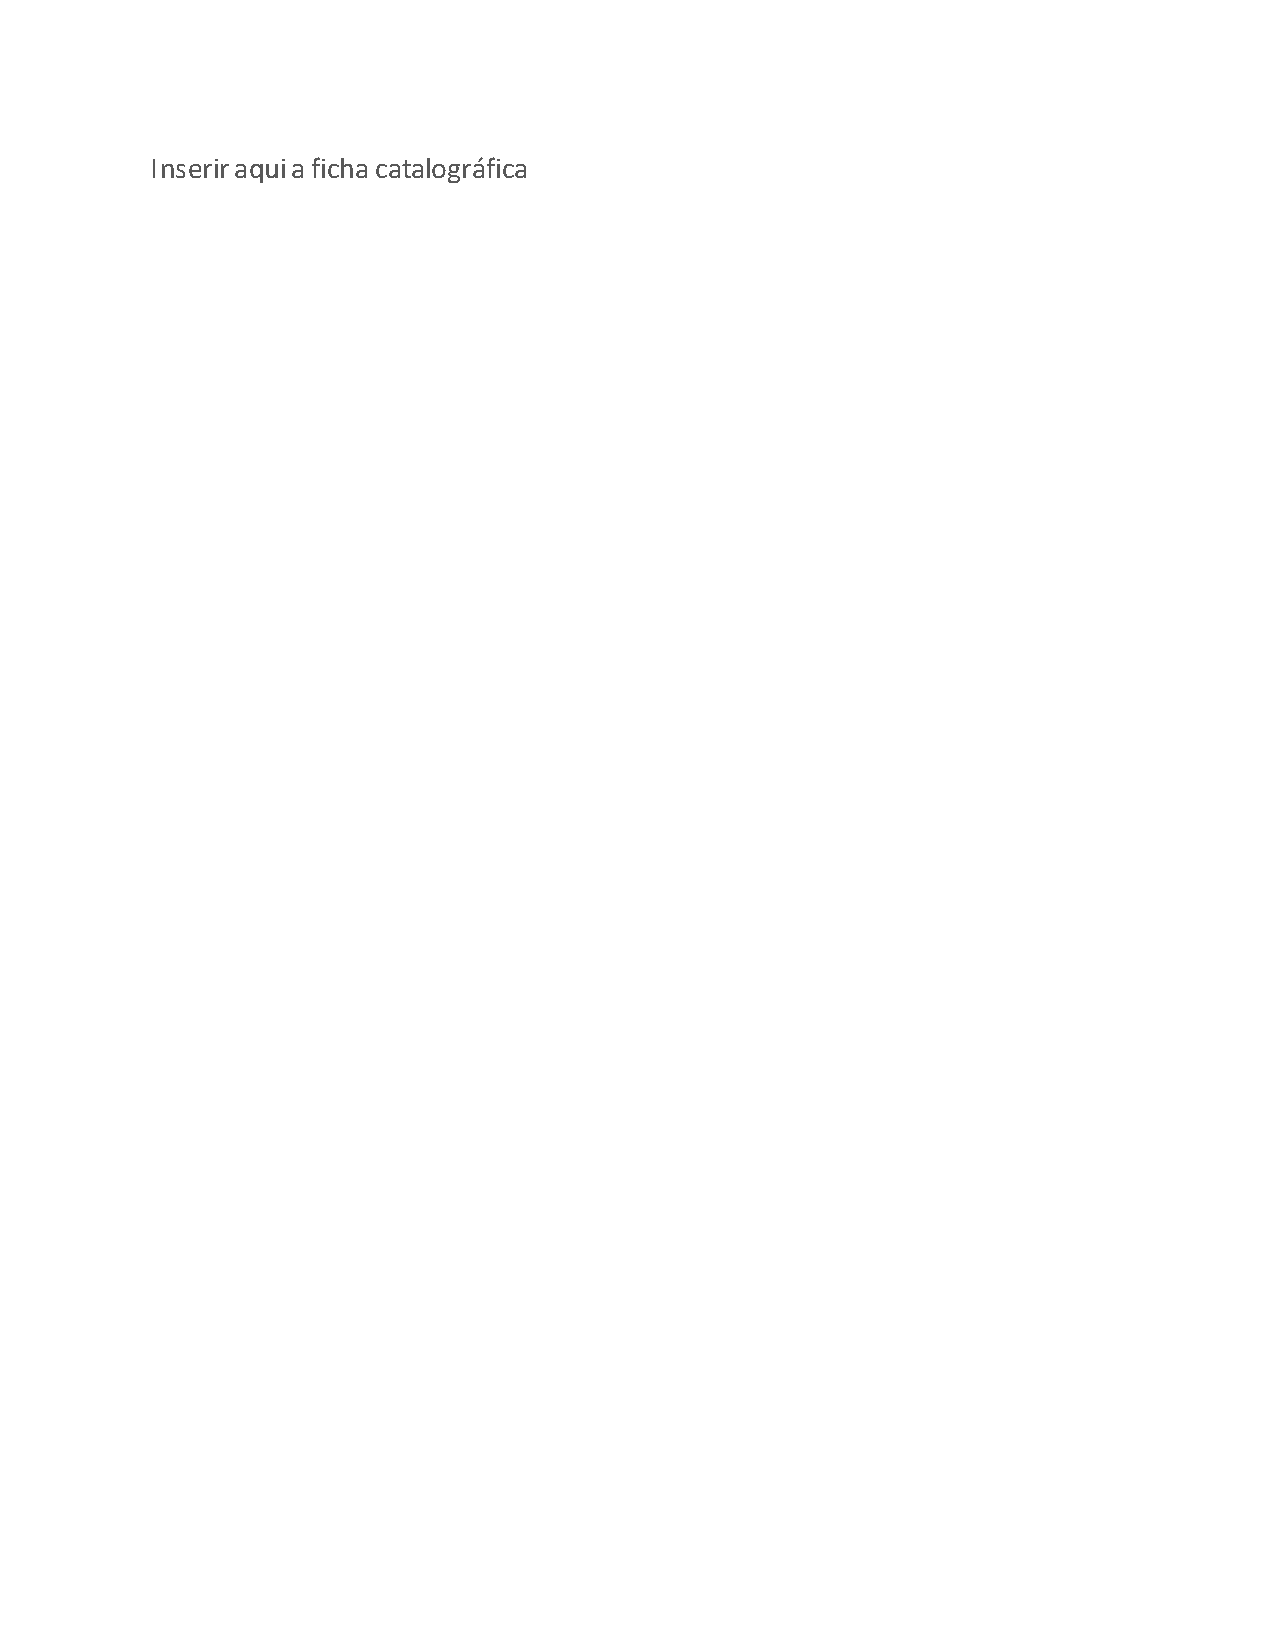
\includepdf{fichaCatalografica/ficha_catalografica}
\end{fichacatalografica}

% Inserir folha de aprovação
% --- para inserir a folha de aprovação retire o % da linha de baixo.
%%
% Este é um exemplo de folha de aprovação.
%
% A folha de aprovação final será inserida pelo Coordenador do Curso.
%

\begin{folhadeaprovacao}
	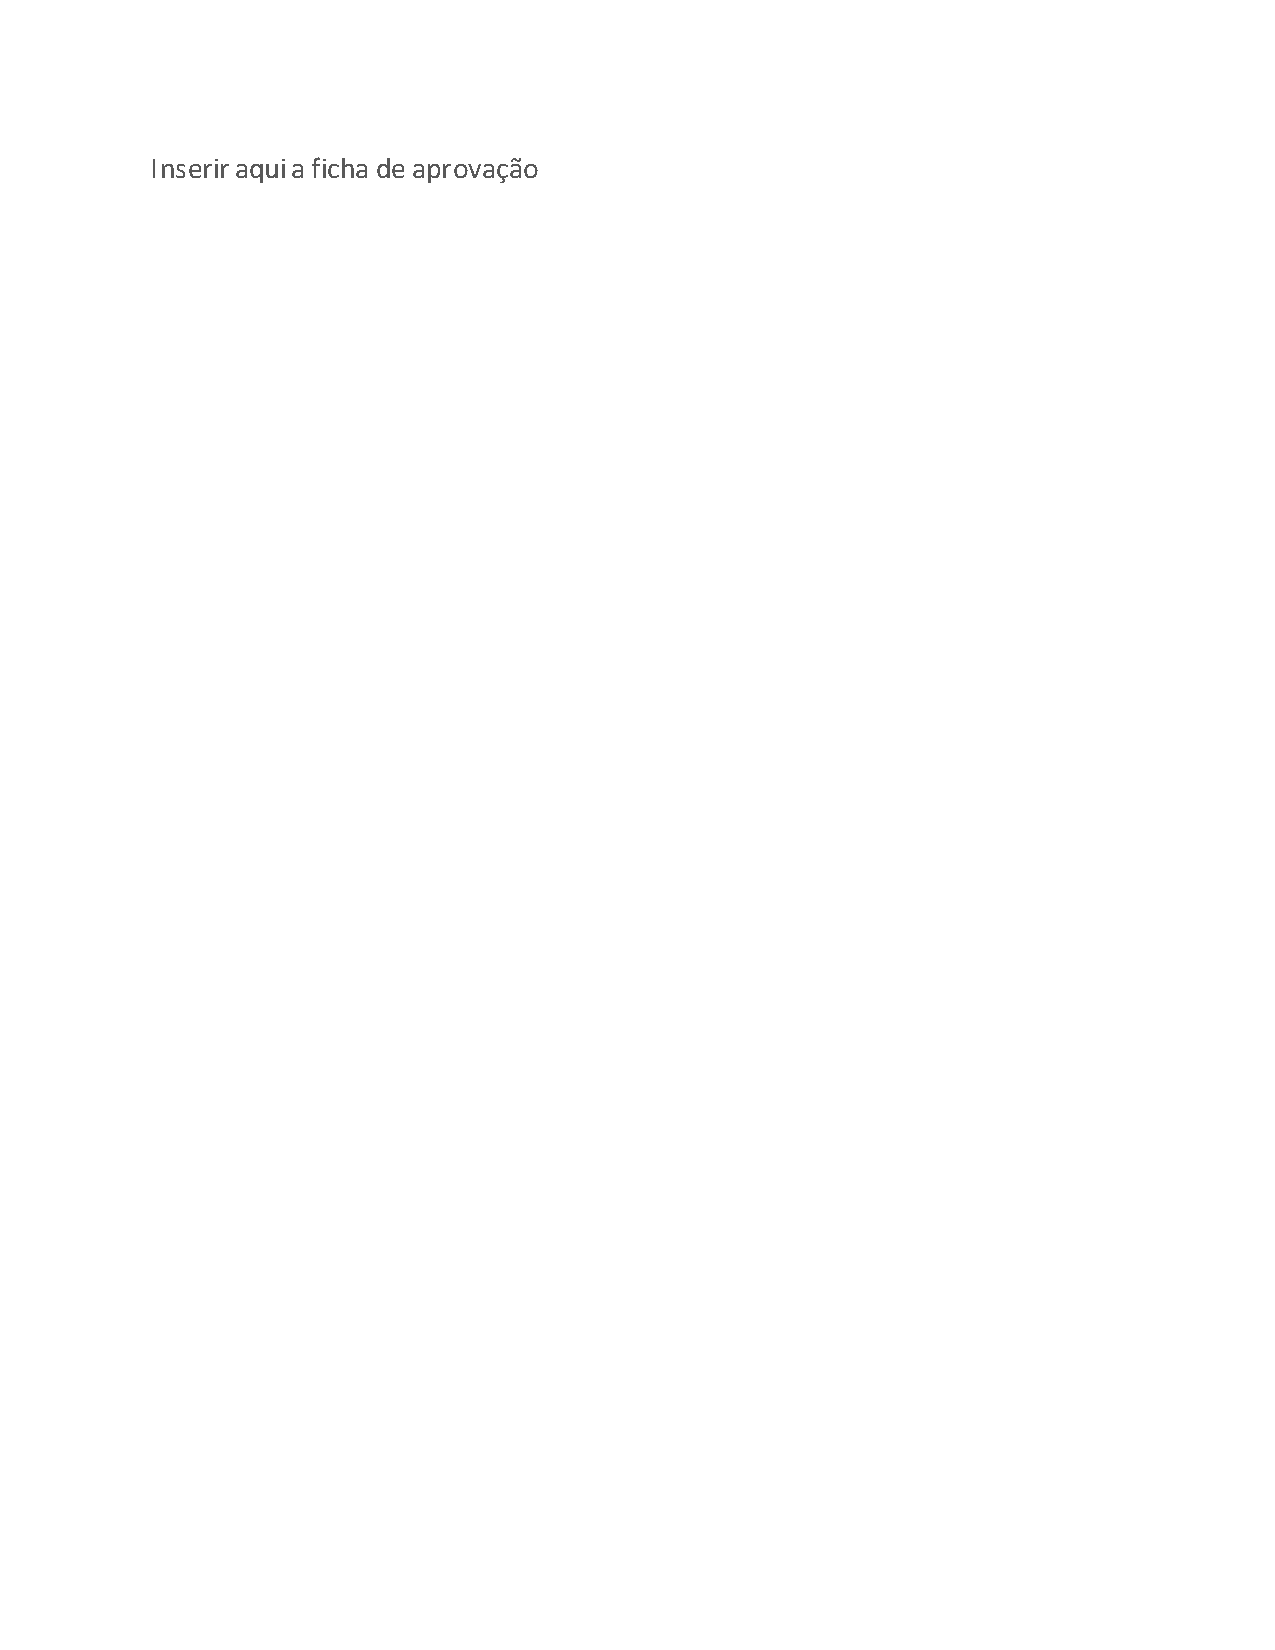
\includepdf{folhaAprovacao/folha_aprovacao}
\end{folhadeaprovacao}
% ---
% Dedicatória
% --- para inserir dedicatória, retire o % da linha de baixo.
% \begin{dedicatoria}
	\vspace*{\fill}
	\centering
	\noindent
	\textit{Dedicatória (Opcional). Não digite a palavra Dedicatória. Texto no qual o autor do trabalho oferece homenagem ou dedica o seu trabalho a alguém (não usar ponto final)}
    \vspace*{\fill}
\end{dedicatoria}
% ---
% Agradecimentos
\begin{agradecimentos}
	A descrição dos agradecimentos é opcional.
	Caso você não deseje inserir agradecimento, já até a página de configuração (monografia\_config) e insira um comentário (\%) na chamada da página.
	
	Caso faça os agradecimentos, se atente em seguir algumas dicas de boa escrita:
	
	\begin{itemize}
	    \item Cite as pessoas que foram responsáveis pela execução do seu trabalho, porém se atente em agradecer brevemente, para não ficar muito extenso;
	    \item Cite a instituição e possíveis recursos utilizados que te ajudaram a terminar o projeto;
	    \item Caso tenha fomento, cite um breve agradecimento;
	    \item Caso resolva fazer agradecimentos pessoais, evite citar muitas pessoas, faça um breve agradecimento de modo geral, para evitar um texto muito carregado;
	    \item Agradeça ao seu orientador e coorientador e outros colaboradores ligados ao projeto;
	    \item Evite expressões tais quais "obrigado por não surtar" ;  "esse TCC me fez passar muito nervoso" , "agradeço aos meus cachorros", "agradeço ao meu psiquiatra que me receitou Rivotril".. TCC é um documento do aluno que será registrado na biblioteca, podendo ser publicado em teses online, portanto, por mais que seja brincadeira, não é legal inserir esse tipo de declaração. Sem contar que a banca pode ter uma impressão negativa de você.
	\end{itemize}
\end{agradecimentos}
% ---
% Epígrafe
% --- para inserir Epígrafe, retire o % da linha de baixo
% \begin{epigrafe}
	
	\vspace*{\fill}
	Epígrafe (Opcional). Pensamentos retirados de um livro, uma música, um poema, normalmente relacionado ao tema do trabalho, seguida de indicação de autoria. As epígrafes podem ser colocadas também nas folhas de abertura de cada capítulo.  
    
	\epigraph{``\emph{Any fool can write code that a computer can understand. Good programmers write code that humans can understand}''.}{Martin Fowler}
	
\end{epigrafe}
% ---
% Resumos
\begin{resumo}

%\noindent{SILVA, João da. \textbf{Título do trabalho de conclusão de curso em negrito}. Nº de fls. TCC (Trabalho de Conclusão de Curso). Instituto Federal de Mato Grosso do Sul – IFMS. Tecnologia em Análise e Desenvolvimento de Sistemas, Câmpus Nova Andradina, MS. 2018.}

%\setlength{\absparsep}{18pt} % ajusta o espaçamento dos parágrafos do resumo
%\vspace{1.5cm}
	
A acessibilidade digital é um desafio crucial em um mundo cada vez mais conectado, especialmente para pessoas com deficiência visual. Este trabalho apresenta o desenvolvimento de um aplicativo multiplataforma assistivo capaz de capturar imagens do ambiente e descrevê-las em áudio, utilizando modelos de linguagem de grande porte (LLMs) de código aberto. O aplicativo integra recursos de visão computacional e síntese de voz (Text-to-Speech - TTS), promovendo maior autonomia para usuários com deficiência visual. A metodologia incluiu o benchmark de três modelos de IA (Qwen 2.5, llava v1.6 Mistral e Llama 3.2 Vision), avaliados com base em métricas de latência, qualidade textual (BERTScore e ROUGE-L) e testes práticos em cenários reais. Os resultados demonstraram que o modelo Qwen 2.5 apresentou o melhor equilíbrio entre precisão descritiva e desempenho em tempo real. O protótipo desenvolvido evidencia o potencial da IA para ampliar a inclusão digital, destacando-se como uma solução inovadora para a melhoria da qualidade de vida de pessoas com deficiência visual.

	\vspace{\onelineskip}
	
	\textbf{Palavras-chave}: Acessibilidade Digital, Tecnologia Assistiva, Modelos de Linguagem Multimodais, Visão Computacional, Inclusão Social.
	
\end{resumo}
\begin{resumo}[Abstract]
	
	\begin{otherlanguage*}{english}
		
	Digital accessibility is a crucial challenge in an increasingly connected world, especially for people with visual impairments. This paper presents the development of a cross-platform assistive application capable of capturing environmental images and describing them in audio using open-source large language models (LLMs). The application integrates computer vision and text-to-speech (TTS) technologies, promoting greater autonomy for visually impaired users. The methodology included benchmarking three AI models (Qwen 2.5, llava v1.6 Mistral e Llama 3.2 Vision), evaluated based on latency metrics, textual quality (BERTScore and ROUGE-L), and practical tests in real-world scenarios. The results showed that the Qwen 2.5 model achieved the best balance between descriptive accuracy and real-time performance. The developed prototype demonstrates the potential of AI to enhance digital inclusion, standing out as an innovative solution to improve the quality of life for visually impaired individuals.
	
    \textbf{Keywords}: Digital Accessibility, Assistive Technology, Multimodal Language Models, Computer Vision, Social Inclusion.
		
	\end{otherlanguage*}

\end{resumo} 
% ---
% inserir lista de ilustrações
% ---
\renewcommand{\listfigurename}{\large{Lista de figuras}}
\pdfbookmark[0]{\listfigurename}{lof}
\listoffigures*  % O * remove esse item do indice
\cleardoublepage
% ---
% inserir lista de tabelas
% ---
\renewcommand{\listtablename}{\large{Lista de Tabelas}}
\pdfbookmark[0]{\listtablename}{lot}
\listoftables*
\cleardoublepage
% ---
% ---
% inserir lista de quadros
% --- Para inserir lista de quadros, tire o % da linha de baixo
% \pdfbookmark[0]{\listofquadrosname}{loq}
% \listofquadros*
% \cleardoublepage
% ---
% inserir lista de abreviaturas e siglas
% --- para inserir lista de Abreviaturas e Siglas, retire o % da linha de baixo
%\begin{siglas}
	\item AAAAAAAAAA
\end{siglas}


%*******************************************************
%                Acronimos
%*******************************************************
    %\phantomsection 
    %\refstepcounter{dummy}
    %\pdfbookmark[1]{Acronyms}{acronyms}
    %\markboth{\spacedlowsmallcaps{Acronyms}}{\spacedlowsmallcaps{Acronyms}}
    %\chapter*{\large{Acrônimos}}
    %\begin{acronym}[UML]
        %\acro{XXX}{nome aqui}
    %\end{acronym} 
    
    %\cleardoublepage
% ---

% ---
% inserir lista de símbolos
% ---
% \begin{simbolos}
	\item[$\alpha$] Letra grega minúscula Alfa
	\item[$\beta$] Letra grega minúscula Beta
\end{simbolos}
% ---

% ------------------------------------
% INSERIR SUMÁRIO
% -----------------------------------
\renewcommand{\contentsname}{\large{SUMÁRIO}}

\pdfbookmark[0]{\contentsname}{toc}
\tableofcontents*
\cleardoublepage
% ---

% ----------------------------------------------
%             ELEMENTOS TEXTUAIS
%           INSERIR NOVOS ARQUIVOS
% ----------------------------------------------
% cada um desses comandos a baixo montam uma seção de capítulos do nosso documentos na hora da compilação.
% note que eles foram chamados com a ordem que eles aparecerão no documento final. Ideal é que no momento da criação, sejam renomeados de maneira lógica, numerando o capítulo e a seção.

\textual
\pagestyle{meuestilo}
\chapter{Introdução}

A acessibilidade digital tem se tornado um tema de crescente importância em um mundo cada vez mais conectado. O desenvolvimento tecnológico, nos últimos anos, tem despertado a atenção do mundo todo, especialmente quando o assunto trata-se de Inteligência Artificial (IA). Porém, mesmo em um mundo conectado, o desenvolvimento de tecnologias assistivas ainda caminha a passos lentos, levando anos para chegarem às pessoas com deficiência, especialmente aos deficientes visuais, que, por não terem visão ou terem, porém, limitada, são prejudicados no contato com recursos inovadores existentes atualmente. 

Segundo dados da \citeonline{WHO2023}, estima-se que pelo menos 2,2 bilhões de pessoas em todo o mundo vivenciam algum grau de deficiência visual, o que ressalta a necessidade de soluções tecnológicas específicas para esse público, visando a melhoria da qualidade de vida e, também, o contato com tecnologias inovadoras, como a IA. No contexto brasileiro, o Instituto Brasileiro de Geografia e Estatística (IBGE) aponta que mais de 6 milhões de pessoas têm algum nível de deficiência visual, o que evidencia a expressividade dessa população, reforçando o caráter urgente de iniciativas que promovam a inclusão. Embora diversos recursos digitais e físicos já existam para auxiliar pessoas cegas ou com baixa visão, ainda há lacunas quanto a ferramentas de reconhecimento de ambientes em tempo real por meio de dispositivos móveis.

Frente a esse cenário, o presente trabalho propõe o desenvolvimento de um aplicativo multiplataforma, capaz de capturar imagens do ambiente e descrevê-las em áudio por meio de técnicas de IA, promovendo a inclusão tecnológica e, além disso, melhorando a qualidade de vida de deficientes visuais. De acordo com \citeonline{silvaneto2024tecnologias}, a IA surge como um meio promissor para ampliar o acesso ao conhecimento, eliminar barreiras e melhorar a experiência acadêmica de grupos historicamente excluídos, como pessoas com deficiência, minorias étnicas e socioeconômicas. Nesse sentido, a proposta está alinhada às demandas atuais de inclusão e às oportunidades tecnológicas propiciadas pela evolução da IA, especialmente ao desenvolvimento dos modelos de linguagem de grande porte (do inglês, Large Language Models - LLMs), onde muitos são disponibilizados de forma gratuita, com o código aberto, em plataformas como o Hugging Face.

Desta forma, dada a crescente popularização dos smartphones e a melhoria contínua dos recursos de câmera embutidos nesses dispositivos, caminhos foram abertos para soluções inovadoras no campo da visão computacional. Não obstante, não podemos encarar a acessibilidade como um recurso adicional da tecnologia, mas como uma parte fundamental do desenvolvimento, visando garantir o acesso a qualquer grupo que a utilize. Assim, o desenvolvimento de aplicativos que traduzem informações visuais em descrições textuais e, posteriormente, em áudio, pode transformar a forma como pessoas com deficiência visual interagem com o ambiente ao seu redor.

A relevância deste estudo decorre do compromisso social de promover inclusão e autonomia a grupos historicamente sub-representados na evolução tecnológica. Além dos dados estatísticos já mencionados, há também uma motivação acadêmica, pois o uso de modelos de código livre de LLM para descrever imagens em tempo real é um tema ainda em consolidação na literatura científica, onde muitos estudos optam por usar modelos já renomados no mercado, porém proprietários. De acordo com \citeonline{lecun2015deeplearning}, o aumento da capacidade computacional, a disponibilidade de grandes bases de dados e o desenvolvimento de ferramentas de análise de dados impulsionam significativamente o progresso em redes neurais profundas, podendo contribuir para existirem modelos cada vez mais robustos. Todavia, ainda há desafios relacionados à latência, ao custo computacional e à efetiva acurácia das legendas geradas.

Assim, ao comparar diferentes modelos de linguagem pré-treinados (por exemplo, Qwen2.5-VL-7B-Instruct, Llama-3.2-11B-Vision-Instruct e o llava-v1.6-mistral-7b-hf), este trabalho busca evidenciar pontos fortes e limitações de cada abordagem, contribuindo para a consolidação de uma prática fundamentada na seleção e no emprego de soluções de IA em projetos de acessibilidade. Desta forma, este trabalho tem como objetivo desenvolver um aplicativo móvel que possibilite a descrição em áudio de elementos do ambiente para pessoas com deficiência visual, valendo-se de um servidor para processamento de imagens por meio de LLMs de código livre. Assim, como resultado final, será desenvolvida uma tecnologia assistiva que poderá contribuir fortemente para a melhoria da qualidade de vida de deficientes visuais e, além disso, proporcionar o uso de tecnologias inovadoras da atualidade.

Para alcançar esse objetivo, este trabalho está detalhado em 5 capítulos, além desta introdução, que buscou apresentar resumidamente sobre a problemática, além de discorrer sobre o objetivo geral do desenvolvimento.

No Capítulo 2, que trata do Referencial Teórico, valeu-se de uma pesquisa detalhada acerca dos conceitos de acessibilidade, tecnologias assistivas, visão computacional e do funcionamento de modelos de linguagem de grande porte, além de explorar brevemente questões sobre Text-to-Speech. Esta foi realizada por meio de ferramentas como o Periódicos Capes, Google Acadêmico e demais repositórios de trabalhos da área. 

Em seguida, no Capítulo 3 é apresentada a Metodologia, onde os métodos, ferramentas e procedimentos adotados para o desenvolvimento do aplicativo, incluindo a estratégia de benchmark dos diferentes modelos de IA, são detalhados. 

Já os Resultados e Discussões, que estão no Capítulo 4, descrevem os resultados obtidos nos testes práticos e no benchmark, analisando as métricas de desempenho e a usabilidade da solução. 

Por fim, a Conclusão, no Capítulo 5, retoma os objetivos iniciais, faz considerações finais sobre o trabalho realizado e sugere futuros aprimoramentos, dando encerramento ao trabalho.


% \chapter{Objetivos}  \label{cap:02}

% Para a Banca Final, lembre-se de conversar com o orientador sobre suprimir esse capítulo já que ele terá sido cumprido, e inserí-lo na Introdução em modo Parágrafo. 
% Não apague esse comentário.


\section{Objetivo Geral}

O objetivo geral do trabalho é o elemento que resume e apresenta a ideia central do trabalho acadêmico. Normalmente é redigido em uma frase, utilizando o verbo no infinitivo. 

% textbf é um comando que deixa o texto em negrito
\textbf{Exemplo:} Detalhar o presente modelo de escrita para a produção do Trabalho de Conclusão de Curso.\\

\section{Objetivos Específicos}

% textit é um comando que deixa o texto em itálico
Os objetivos específicos definem os diferentes pontos a serem abordados, visando confirmar as hipóteses e concretizar o objetivo geral. Em suma, são as ações que serão desenvolvidas a fim de que se alcance o \textit{objetivo geral}. Devem ser escritos no infinitivo.

\textbf{Exemplo:}

\begin{itemize}
    \item Realizar a revisão bibliográfica sobre TCC;
    \item Criar um Tutorial sobre a utilização do Overleaf;
    \item Aplicar os conhecimentos adquiridos para edição de documentos.
\end{itemize}
\chapter{Referencial Teórico}  \label{cap:02}

O referencial teórico tem como objetivo fundamentar este estudo a partir de conceitos e pesquisas já consolidadas na literatura científica. Por meio da revisão de trabalhos acadêmicos, artigos e documentos técnicos, esta seção apresenta as principais bases conceituais relacionadas ao desenvolvimento deste projeto.

Inicialmente, são abordados aspectos fundamentais sobre acessibilidade e deficiência visual, destacando a importância da tecnologia assistiva para promover inclusão social. Em seguida, discutem-se as principais tecnologias de apoio utilizadas atualmente, incluindo soluções baseadas em visão computacional e inteligência artificial. Também são explorados conceitos relacionados a LLMs e sua aplicação na descrição automática de imagens, além de métricas de avaliação da qualidade das descrições geradas.

Por fim, são detalhadas as tecnologias de reconhecimento e síntese de fala (\textit{Speech-to-Text} e \textit{Text-to-Speech}), essenciais para a interface acessível do sistema proposto. Essas discussões servirão como base para a construção e análise do modelo desenvolvido, garantindo alinhamento com os avanços mais recentes na área.

\section{Acessibilidade e Deficiência Visual}

A acessibilidade digital refere-se à capacidade de indivíduos, independentemente de suas habilidades ou deficiências, acessarem e interagirem com informações e serviços disponíveis no ambiente digital. \citeonline{Torres2002} destacam que a acessibilidade no espaço digital envolve a adaptação de conteúdos e interfaces para garantir que pessoas com diferentes tipos de deficiência possam utilizá-los de forma eficaz.

No contexto das pessoas com deficiência visual, a acessibilidade digital é particularmente desafiadora. Conforme destacam \citeonline{Torres2002}, “as barreiras arquitetônicas não são o maior obstáculo enfrentado pelas pessoas portadoras de deficiência. O maior obstáculo está no acesso à informação e, consequentemente, a aspectos importantes relacionados à informação, como a educação, o trabalho e o lazer”. Desta forma, é evidente que se fazem necessárias melhorias nas tecnologias existentes para a distribuição e acesso das pessoas deficientes, como dito por \citeonline{romeo2019}, que analisam o uso de diferentes tecnologias para acesso a conteúdos digitais por pessoas com deficiência visual e sugerem melhorias nas recomendações existentes para a concepção de \textit{websites} acessíveis. Deste modo, com a evolução não somente dos \textit{websites}, mas também de todas as tecnologias, a melhoria da acessibilidade para as pessoas deficientes seria nítida.

\subsection{Dados e Estatísticas sobre a População com Deficiência Visual}

Compreender a dimensão da população com deficiência visual é crucial para justificar a relevância de soluções tecnológicas acessíveis, para que, como exposto anteriormente, a acessibilidade em ambientes digitais passe por uma melhora significativa e contribua para o acesso de todos os grupos da sociedade. \citeonline{Castro2008} conduziram um estudo que descreve a prevalência e os fatores associados às deficiências visuais, auditivas e físicas no Brasil, constatando que 68\% do público entrevistado possuía algum tipo de deficiência visual, sendo a dificuldade de enxergar a principal deficiência referida e, como um dos principais fatores agravantes, o envelhecimento, conforme apresentado pelos autores. Fica claro, portanto, que este público merece atenção redobrada, dado que, segundo o \citeonline{ibgecenso2022}, em 2022 o índice de envelhecimento da população brasileira chegou a 80,0, indicando que há 80 pessoas idosas para cada 100 crianças de 0 a 14 anos, mas, comparado a 2010, o índice de envelhecimento era menor, correspondendo a 44,8, evidenciando um aumento de 78,5\%. Esses números corroboram para que a acessibilidade digital seja um ponto de discussão sério e fundamental para o desenvolvimento da inclusão digital.

Além disso, o IBGE tem desempenhado um papel fundamental na coleta e análise de dados relacionados à população com deficiência no Brasil. A produção e divulgação dessas informações são essenciais para embasar políticas públicas e iniciativas voltadas à inclusão social. A coleta de informações ocorre por meio de pesquisas como a Pesquisa Nacional de Saúde (PNS) de 2019, a Pesquisa Nacional por Amostra de Domicílios Contínua (PNAD Contínua) de 2022 e o Censo Demográfico, cada uma com metodologias e objetivos específicos. Segundo \citeonline{Botelho2024}, “as pesquisas conduzidas pelo IBGE adotam as recomendações do Grupo de Washington de Estatísticas sobre Deficiência, mas empregam questionários distintos, o que demanda atenção dos usuários desses dados”. Esse fator evidencia a complexidade na interpretação dos indicadores e destaca a necessidade de critérios padronizados para garantir a comparabilidade ao longo do tempo. O artigo também ressalta que as pessoas com dificuldades mais severas são as que enfrentam os maiores desafios no acesso à educação e ao mercado de trabalho, o que reforça a importância de políticas públicas baseadas em dados precisos. Tais informações são fundamentais não apenas para o desenvolvimento de políticas sociais, mas também para a criação de tecnologias assistivas que possam atender às demandas dessa parcela da população.

\subsection{Panorama de Leis e Normas}

A legislação brasileira tem avançado significativamente na promoção da inclusão e acessibilidade para pessoas com deficiência visual, estabelecendo diretrizes que garantem o acesso igualitário a diversos aspectos da vida em sociedade, incluindo a educação, o trabalho e o lazer. A Lei Brasileira de Inclusão da Pessoa com Deficiência (Lei nº 13.146/2015), também conhecida como Estatuto da Pessoa com Deficiência, representa um marco regulatório importante, pois estabelece diretrizes para garantir acessibilidade em diversas esferas, incluindo educação, transporte, comunicação e tecnologia. Segundo \citeonline{Bruno2019}, a política nacional de inclusão digital tem se mostrado essencial para eliminar barreiras atitudinais e tecnológicas, proporcionando autonomia e participação ativa na sociedade para pessoas com deficiência visual. A acessibilidade digital, nesse contexto, é reconhecida como um direito fundamental, assegurando que todos os cidadãos tenham acesso igualitário às informações e oportunidades disponíveis no ambiente digital.

Além disso, a Política Nacional de Educação Especial na Perspectiva da Educação Inclusiva \cite{Brasil2008} reforça o papel da tecnologia assistiva como um recurso essencial para a inclusão educacional de pessoas com deficiência visual. O decreto nº 7.611/2011, que regulamenta a educação especial, define o Atendimento Educacional Especializado (AEE) como um conjunto de recursos e estratégias pedagógicas voltadas para a eliminação de barreiras ao aprendizado, com a implementação de salas de recursos multifuncionais equipadas com tecnologia assistiva específica, como softwares de leitura de tela e impressoras em braille. Essas iniciativas, no entanto, ainda enfrentam desafios quanto à implementação efetiva em diferentes níveis de ensino, conforme destacado por \citeonline{CHILINGUE2024}, que aponta que a ausência de adequação em ambientes virtuais de aprendizagem compromete a inclusão digital plena de estudantes com deficiência visual. Assim, embora haja avanços legislativos e normativos, a acessibilidade digital e educacional ainda requer esforços contínuos para garantir que as políticas sejam aplicadas de forma abrangente e eficaz.

Esses marcos legais reforçam a importância de desenvolver tecnologias assistivas que promovam a acessibilidade digital, garantindo que pessoas com deficiência visual possam exercer plenamente seus direitos e participar ativamente da sociedade.

\section{Tecnologias de Apoio}

As tecnologias assistivas desempenham um papel essencial na promoção da inclusão de pessoas com deficiência visual, permitindo-lhes superar barreiras e interagir de maneira mais autônoma com o mundo ao seu redor. Como visto anteriormente, aproximadamente 2,2 bilhões de pessoas em todo o mundo possuem algum grau de deficiência visual, sendo que uma parcela significativa enfrenta desafios na locomoção, acesso à informação e comunicação \cite{WHO2023}. A introdução de tecnologias assistivas tem proporcionado avanços significativos, melhorando a qualidade de vida e promovendo a equidade de acesso em diversos contextos, como a educação e o mercado de trabalho.

\subsection{Tecnologias Assistivas e sua Contribuição}

O termo Tecnologia Assistiva é utilizado para identificar todo o arsenal de recursos e serviços que contribuem para proporcionar ou ampliar habilidades funcionais de pessoas com deficiência e, consequentemente, promover vida independente e inclusão \cite{bersch2024}. Segundo \citeonline{silvaneto2024tecnologias}, a adoção dessas tecnologias tem sido crucial para garantir a acessibilidade digital, proporcionando autonomia no uso de computadores e dispositivos móveis por meio de recursos como leitores de tela e aplicativos de reconhecimento de imagem.

A utilização dessas ferramentas contribui significativamente para a inclusão de pessoas com deficiência visual em ambientes educacionais, profissionais e sociais. Conforme destacado em um estudo de \citeonline{BORGES2021}, o uso de softwares assistivos tem por finalidade eliminar as barreiras à plena participação e à vida funcional para as pessoas com deficiência, incapacidades e mobilidade reduzida, objetivando uma maior autonomia e qualidade de vida. Portanto, pode-se notar a importância destes dispositivos atualmente, principalmente dos \textit{smartphones} e outros dispositivos populares, dado o fácil acesso de toda a população, inclusive da parcela desfavorecida visualmente. Ademais, a inclusão digital e social dessas pessoas é fortalecida por iniciativas que combinam políticas públicas e o avanço tecnológico, promovendo um ambiente mais inclusivo e acessível, contribuindo ainda mais para o acesso à informação deste grupo.

\subsection{Aplicações Existentes}

Atualmente, diversas aplicações tecnológicas foram desenvolvidas para atender às necessidades das pessoas com deficiência visual, proporcionando maior autonomia em atividades do cotidiano. Essas tecnologias englobam desde soluções simples, como leitores de tela, até dispositivos mais avançados, como bengalas eletrônicas equipadas com sensores ultrassônicos. A seguir, são apresentados alguns exemplos de tecnologias assistivas que vêm sendo amplamente utilizadas:

\begin{enumerate}
    \item \textbf{Leitores de Tela:} Softwares que convertem texto digital em áudio, permitindo que os usuários acessem conteúdos online, documentos e aplicativos. Estudos demonstram que leitores de tela são ferramentas fundamentais para inclusão digital, proporcionando acesso equitativo à informação \cite{brilli2024}. Exemplos incluem:
        \begin{enumerate}
            \item NVDA (NonVisual Desktop Access): Software de código aberto, amplamente utilizado, compatível com múltiplos sistemas operacionais;
            \item JAWS (Job Access With Speech): Um dos leitores de tela mais completos, com suporte a diversas funcionalidades avançadas.
        \end{enumerate}
    \item \textbf{Aplicativos de Descrição de Imagens:} Aplicativos baseados em inteligência artificial capazes de analisar imagens e fornecer descrições detalhadas por meio de síntese de voz. Essas soluções ajudam os usuários a identificar objetos, reconhecer pessoas e entender contextos visuais. Segundo \citeonline{silvaneto2024tecnologias}, tais aplicativos têm demonstrado impacto significativo na autonomia de pessoas com deficiência visual. Exemplos notáveis:
        \begin{enumerate}
            \item Seeing AI (Microsoft): “Aplicativo móvel que fornece recursos de leitura de texto, moeda, produto, reconhecimento facial e descrição de cena” \cite{Dognin2022};
            \item Envision AI: Aplicativo que permite capturar imagens e obter descrições precisas em áudio.
        \end{enumerate}
    \item \textbf{Bengalas Eletrônicas:} As bengalas eletrônicas utilizam sensores de proximidade e \textit{feedback} hápticos para ajudar os usuários a detectar obstáculos no caminho. As localizações bem estudadas dos sensores utilizados permitem a locomoção segura e confortável do usuário, já que toda a cena à sua frente, do topo ao chão, é interpretada \cite{AmmarBouhamed2012}. Dispositivos como:
        \begin{enumerate}
            \item WeWALK: Uma bengala equipada com sensores ultrassônicos e integração com assistentes virtuais;
            \item UltraCane: Tecnologia baseada em sensores de eco para navegação segura em ambientes urbanos.
        \end{enumerate}
    \item \textbf{Softwares de OCR (Reconhecimento Óptico de Caracteres):} Conforme proposto por \citeonline{Sonth2017}, são aplicações capazes de realizar a conversão eletrônica de imagens em texto codificado por máquina, podendo, posteriormente, aplicar técnicas de síntese de voz para o apoio às pessoas com desafios visuais. Essas ferramentas são amplamente utilizadas para leitura de documentos físicos, proporcionando maior independência aos usuários. Exemplos incluem:
        \begin{enumerate}
            \item Google Lens: Reconhece e traduz textos a partir de imagens capturadas com a câmera do \textit{smartphone}.
            \item KNFB Reader: “[...] Mecanismo de OCR que funciona em um telefone celular e permite que uma pessoa com deficiência visual leia texto impresso de uma imagem tirada pela câmera” \cite{wang2010}.
        \end{enumerate}
    \item \textbf{Dispositivos Vestíveis Inteligentes:} A nova geração de tecnologias assistivas inclui dispositivos vestíveis que combinam sensores e inteligência artificial para fornecer informações contextuais sobre o ambiente. Estudos recentes mostram, conforme apontado por \citeonline{brilli2024} que esses dispositivos oferecem uma experiência mais intuitiva e personalizada, ampliando a interação com o ambiente. Exemplos incluem:
        \begin{enumerate}
            \item AIris: De acordo com Brilli et al. (2024):
                \begin{quote}
                    Um dispositivo vestível alimentado por IA que fornece recursos de conscientização e interação ambiental para usuários com deficiência visual. O AIris combina uma câmera sofisticada montada em óculos com uma interface de processamento de linguagem natural, permitindo que os usuários recebam descrições auditivas em tempo real de seus arredores.
                \end{quote}
            \item Envision Glasses: Óculos equipados com reconhecimento de texto e objetos para fornecer feedback auditivo detalhado.
        \end{enumerate}
\end{enumerate}


A \autoref{tab:tecnologiasassistivas} apresenta um resumo de algumas das principais tecnologias assistivas disponíveis para pessoas com deficiência visual, destacando suas funcionalidades e exemplos de aplicação.


\begin{table}[h!]
\centering
\caption{Tecnologias assistivas para deficientes visuais}
\label{tab:tecnologiasassistivas}
\resizebox{\columnwidth}{!}{%
\begin{tabular}{@{}lllll@{}}
\toprule
\textbf{Tecnologia Assistiva} &
  \multicolumn{1}{c}{\textbf{Descrição}} &
  \multicolumn{1}{c}{\textbf{Exemplos}} &
   &
   \\ \midrule
Leitores de Tela &
  Convertam texto digital em áudio ou braille, permitindo acesso a conteúdos online &
  NVDA, JAWS &
   &
   \\
Aplicativos de Descrição de Imagem &
  Utilizam IA para descrever imagens e identificar objetos em tempo real &
  Seeing AI, Envision AI &
   &
   \\
Bengalas Eletrônicas &
  Ajudam na navegação com sensores para detectar obstáculos e fornecer feedback tátil/auditivo &
  WeWALK, UltraCane &
   &
   \\
Softwares de OCR &
  Transformam imagens de textos impressos em texto digital para leitura em voz alta. &
  Google Lens, KNFB Reader &
   &
   \\
Dispositivos Vestíveis Inteligentes &
  Equipamentos que combinam sensores e inteligência artificial para fornecer informações contextuais sobre o ambiente. &
  AIris, Envision Glasses &
   &
   \\ \bottomrule
\end{tabular}%
}
\centering \footnotesize{\textbf{Fonte:} Elaborado pelo Autor (2025)} 
\end{table}

Em suma, as tecnologias assistivas para pessoas com deficiência visual têm desempenhado um papel crucial na promoção da inclusão social e digital. A evolução contínua dessas ferramentas, aliada a iniciativas governamentais e privadas, pode contribuir significativamente para a construção de uma sociedade mais acessível e equitativa.

\section{Visão Computacional}
 
“A visão computacional é o empreendimento de automatizar e integrar uma ampla gama de processos e representações usadas para a percepção da visão” \cite{Ballard1982}. Deste modo, a visão computacional tem como objetivo capacitar máquinas a interpretarem e analisarem informações visuais de forma automatizada, com o objetivo de aproximar-se da percepção humana. De acordo com \citeonline{szeliski2021}:

\begin{citacao}
    Na última década, assistimos a avanços incríveis no desempenho e na confiabilidade dos algoritmos de visão computacional, trazidos em parte pela mudança para o aprendizado de máquina e o treinamento em grandes conjuntos de dados do mundo real.
\end{citacao}

Deste modo, esse grande avanço nas últimas décadas tem contribuído para o surgimento de diversas aplicações inovadoras no ramo da visão computacional, como reconhecimento de imagens, veículos autônomos, monitoramento de segurança, diagnóstico médico e acessibilidade para pessoas com deficiências, proporcionando uma melhor qualidade de vida.

A visão computacional engloba diversas técnicas para a aquisição, processamento, análise e compreensão de imagens digitais. Um dos principais avanços que impulsionou essa área foi o desenvolvimento das Redes Neurais Convolucionais (CNNs), que se tornaram a base para tarefas como classificação de imagens, detecção de objetos e segmentação de imagens, assim como abordado no estudo de \citeonline{LeCun2015}, que traz inúmeros estudos sobre as aplicações das CNNs, desde a identificação e classificação de imagens a aplicações em carros autônomos e tecnologias mais recentes. “As Redes Neurais Convolucionais revolucionaram esse campo aprendendo as formas básicas nas primeiras camadas e evoluindo para aprender características da imagem nas camadas mais profundas, resultando em uma classificação de imagem mais precisa” \cite{Jogin2018}.

O campo da visão computacional é bem amplo, possuindo inúmeras operações que são utilizadas para a melhoria do resultado almejado, como melhores classificações, reconhecimento mais preciso e descrições melhores das imagens. Para alcançar essa melhoria, uma das operações que são essenciais é a de processamento de imagens. “O processamento de imagens envolve processar ou alterar uma imagem existente da maneira desejada” \cite{Phillips1994}. Essas operações são cruciais para melhorar a qualidade das imagens e facilitar a extração de informações relevantes para análise posterior, como exemplificado por \citeonline{szeliski2021}, alguns casos dessas operações são correção de exposição e equilíbrio de cores, redução do ruído da imagem, aumento da nitidez ou rotação das imagens. É possível notar em diversos trabalhos, como o de \citeonline{gonzalez2018} e \citeonline{szeliski2021}, que o processamento de imagens é um pré-requisito fundamental quando se trata de aplicações que as utilizarão. Desta forma, em toda e qualquer aplicação envolvendo a utilização de imagens, é importante aplicar uma camada de processamento para a melhoria e eficácia da aplicação, principalmente quando o aprendizado de máquina está envolvido.

Nos últimos anos, o desenvolvimento de algoritmos mais avançados tem permitido a criação de modelos mais precisos e robustos. Por exemplo, arquiteturas como ResNet \cite{He2015}, EfficientNet \cite{tan2019} e Vision Transformers \cite{dosovitskiy2020} têm demonstrado desempenho superior em \textit{benchmarks} de visão computacional, fornecendo soluções mais eficazes para uma ampla gama de aplicações.

\subsection{Image Captioning}

Com o avanço da legendagem de imagens, também conhecida como \textit{Image Captioning}, inúmeras aplicações voltadas para acessibilidade vêm surgindo, como aplicativos que descrevem ambientes para pessoas com deficiência visual. Seguindo a definição de \citeonline{Hossain2019}:

\begin{citacao}
    A legendagem de imagens é uma área de pesquisa popular da inteligência artificial (IA) que lida com a compreensão da imagem e uma descrição da linguagem para essa imagem. A compreensão de imagens envolve detectar e reconhecer objetos, bem como compreender o tipo ou localização da cena, as propriedades dos objetos e suas interações. Gerar frases bem formadas requer compreensão sintática e semântica da linguagem.
\end{citacao}

Modelos de última geração utilizam uma abordagem multimodal, combinando modelos de visão como CLIP (Contrastive Language-Image Pretraining) com modelos de linguagem, possibilitando a associação correta das legendas com as imagens. Isto é reforçado por \citeonline{radford2021}, onde é apresentado o treinamento de um modelo de \textit{image captioning}, mais especificamente, o CLIP, que é treinado a partir da junção de um codificador de imagem e um codificador de texto para prever os pares corretos de um lote de treinamento, ou seja, ser capaz de identificar com maior precisão os textos associados às imagens. Utilizando o trabalho de \citeonline{Hossain2019} é possível entender melhor como esse processo de junção de um codificador de imagem e um codificador de texto funciona, conforme detalhado na arquitetura apresentada na Figura \ref{fig:1}.


\begin{figure}[!h]
     \caption{Arquitetura da abordagem multimodal de treinamentos de modelos de \textit{image captioning}}
     \centering
     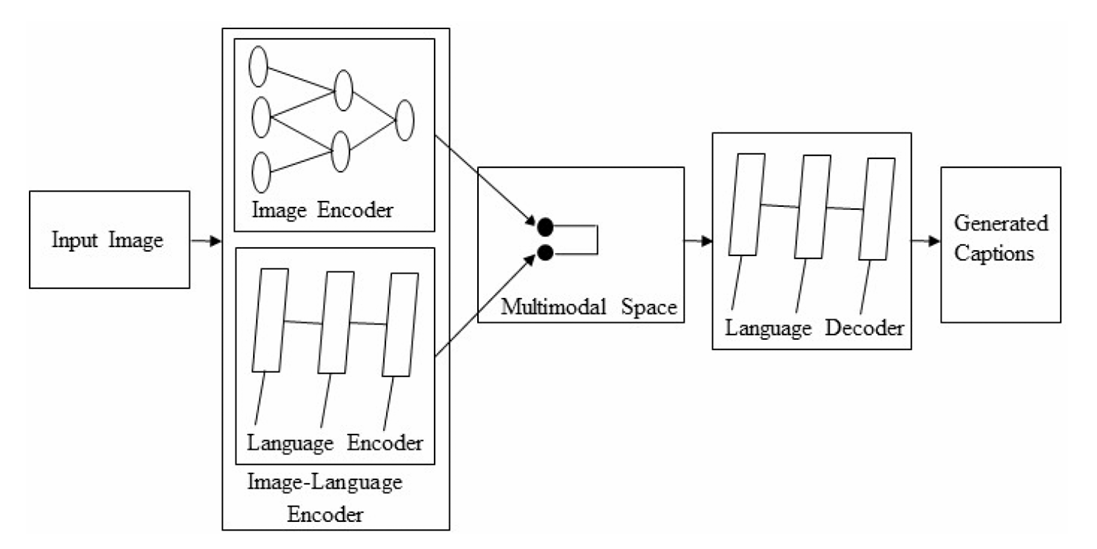
\includegraphics[width=0.7\linewidth]{imagens/treinamento-image-captiong.png}
     \label{fig:1}
     %\footnote{\textbf{Fonte:} \cite{Hossain2019}}
\end{figure}

Desta forma, podemos observar que os codificadores (\textit{Image} e \textit{Language Encoder}) estão juntos, fornecendo entradas para construir o \textit{Multimodal Space}, onde as imagens são associadas com a respectiva legenda para, posteriormente, retornarem as informações. Fazendo o uso de uma descrição mais detalhada:

\begin{citacao}
    A parte de visão [\textit{Image Encoder}] usa uma rede neural convolucional profunda como extrator de recursos para extrair os recursos da imagem. A parte do codificador de linguagem [\textit{Language Encoder}] extrai os recursos da palavra e aprende uma incorporação densa de recursos para cada palavra. Em seguida, encaminha o contexto temporal semântico para as camadas recorrentes. A parte do espaço multimodal [\textit{Multimodal Space}] mapeia os recursos da imagem em um espaço comum com a palavra recursos. \cite{Hossain2019}    
\end{citacao}

A integração dessas tecnologias permite avanços significativos em diferentes tipos de aplicações, incluindo voltadas para o tema de tecnologias assistivas, fornecendo suporte para usuários com deficiência visual por meio da descrição automatizada de ambientes e objetos. 

\section{Modelos de Linguagem de Grande Porte (LLMs)}

Nos últimos anos, um dos desenvolvimentos mais notáveis da área de IA foram os LLMs, que permitem processar e gerar linguagem natural de forma cada vez mais sofisticada. Como destacado por \citeonline{bala2024}, a multimodalidade tem se tornado uma área de pesquisa importante dentro do campo de LLMs, com o objetivo de criar modelos capazes de integrar informações de diferentes modalidades, como texto, imagem e áudio. Essa capacidade de integrar diferentes tipos de dados é crucial para aplicações que utilizem mais de uma forma de entrada, como o proposto neste trabalho, que exige a compreensão de imagens para gerar descrições em linguagem natural.

Os LLMs são modelos de inteligência artificial treinados em conjuntos massivos de dados de texto e código, sendo capazes de compreender e gerar linguagem natural com alto nível de coerência e contexto.  Eles se baseiam em arquiteturas de redes neurais profundas, como os Transformers \cite{vaswani2017}, que revolucionaram o campo do Processamento de Linguagem Natural (PLN). Segundo \citeonline{vaswani2017}, essa arquitetura "evita a recorrência e, em vez disso, se baseia inteiramente em um mecanismo de atenção para estabelecer dependências globais entre a entrada e a saída”. 


\begin{figure}[!h]
     \caption{Arquitetura do modelo Transformer}
     \centering
     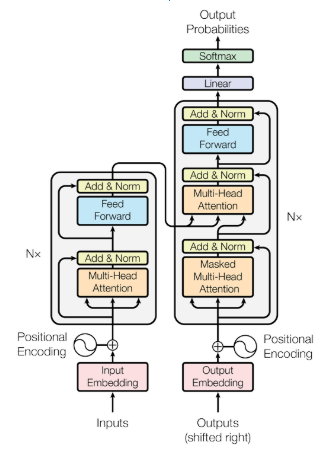
\includegraphics[width=0.7\linewidth]{imagens/transformers.png}
     \label{fig:2}
     %\footnote{\textbf{Fonte:} \cite{vaswani2017}}
\end{figure}

A arquitetura do Transformer é composta por duas redes neurais principais: o codificador (\textit{encoder}) e o decodificador (\textit{decoder}). Como ilustrado na Figura \ref{fig:2}, cada uma dessas redes é estruturada em múltiplas camadas idênticas empilhadas, onde:

\begin{itemize}
    \item \textbf{Codificador:} Recebe a sequência de entrada, aplica \textit{embeddings} e incorpora informações posicionais. Cada camada contém um bloco de \textit{multi-head self-attention}, seguido por uma camada \textit{feed-forward}. O mecanismo de normalização residual (\textit{Add \& Norm}) mantém a estabilidade do treinamento.
    \item \textbf{Decodificador:} Similar ao codificador, mas incorpora uma camada adicional de \textit{Masked Multi-Head Attention}, que impede o modelo de olhar para \textit{tokens} futuros durante a geração de texto. Após essa etapa, as informações passam pelo mecanismo de atenção cruzada (\textit{cross-attention}), que permite ao decodificador utilizar os estados do codificador para refinar a saída.
\end{itemize}

Na última camada do decodificador, os vetores de saída são projetados para probabilidades através de uma camada linear e \textit{softmax}, que gera a predição final da sequência.

A principal inovação do Transformer está no uso da \textit{Multi-Head Attention}, que permite que diferentes partes da entrada sejam analisadas simultaneamente sob diversas perspectivas. Essa abordagem permite que os modelos lidem com sequências de texto de maneira mais eficiente e paralela, superando limitações anteriores encontradas em redes recorrentes. Sendo assim, a arquitetura Transformers foi um marco para o campo de IA, tornando-se a base para os modelos de LLM mais avançados.

De acordo com \citeonline{devlin2018} e \citeonline{thoppilan2022}, modelos como o GPT (Generative Pre-trained Transformer), BERT (Bidirectional Encoder Representations from Transformers) e LaMDA (Language Model for Dialogue Applications) impulsionaram avanços significativos em diversas tarefas de NLP (Natural Language Processing), como geração de texto, tradução automática, resumo automático e resposta a perguntas. O modelo BERT, por exemplo, introduziu uma abordagem bidirecional que melhora a compreensão contextual das palavras em um texto, enquanto o GPT demonstrou avanços notáveis na geração de texto fluente e coerente. O modelo LaMDA, por sua vez, foi projetado para diálogos naturais, possibilitando interações mais humanizadas e relevantes. Esses avanços mostram o impacto dos LLMs na automação de tarefas cognitivas complexas, oferecendo soluções inovadoras para aplicações comerciais, educacionais e de acessibilidade.

\subsection{LLMs Multimodais}

Os modelos de LLM Multimodais, ou MLLM (Multimodal Large Language Model) são uma evolução significativa dos modelos de linguagem, projetados para processar e gerar informações a partir de diferentes tipos de dados, como texto, imagens e áudio. Da mesma forma que destacado por \citeonline{bala2024}, também é notável a importância destes avanços pelo trabalho de \citeonline{wu2023}:

\begin{citacao}
    O nosso mundo é inerentemente multimodal e os seres humanos percepcionam o mundo com diferentes órgãos sensoriais para informação modal variada, como a linguagem, as imagens, os vídeos e os sons, que muitas vezes se complementam e sinergizam entre si. Com esta intuição, os LLM puramente baseados em texto foram recentemente dotados de outras capacidades de compreensão e de percepção de imagem, vídeo, áudio, etc.
\end{citacao}

Desta forma, modelos como o CLIP, citado no trabalho de \citeonline{radford2021}, demonstram a capacidade de conectar imagens e texto de forma eficaz, aprendendo a representar ambos em um espaço vetorial compartilhado. Essa capacidade permite ao CLIP realizar tarefas como  \textit{zero-shot image classification}, geração de legendas para imagens e  busca de imagens a partir de descrições textuais.

O CLIP é um dos exemplos de modelos que existem com a capacidade multimodal, mas existem vários outros, como o NExT-GPT \cite{wu2023} e o LLaVA \cite{liu2023}. A extensão de modelos MLLM nos últimos anos vem crescendo exponencialmente, como pode-se notar na Figura \ref{fig:3}, elaborada por \citeonline{Yin2024}, evidenciando uma linha do tempo dos MLLMs.

\begin{figure}[!h]
     \caption{Modelos MLLMs existentes}
     \centering
     \includegraphics[width=0.7\linewidth]{imagens/avanços-llms.png}
     \label{fig:3}
     \footnote{\textbf{Fonte:} \cite{Yin2024}}
\end{figure}

Em suma, os MLLMs representam uma inovação significativa no campo da inteligência artificial, proporcionando uma compreensão mais abrangente dos dados por meio da integração de múltiplas modalidades. Por fim, fica claro que a gama de modelos possíveis para a utilização é alta, viabilizando diversas aplicações inovadoras que envolvem vários tipos de entrada, voltadas para acessibilidade, automações e outras áreas equivalentes.

\subsection{LLMs e MLLMs \textit{Open Source}}

Os LLMs e MLLMs de código aberto oferecem vantagens significativas para pesquisadores, desenvolvedores e organizações que buscam soluções avançadas em inteligência artificial. Uma plataforma central nesse ecossistema é a Hugging Face, que se destaca como um repositório líder para modelos de código aberto.

\begin{citacao}
    Hugging Face (HF) e seu Hub se destacam nesse aspecto [pesquisa e desenvolvimento de IA] devido ao seu papel crítico no desenvolvimento, compartilhamento e implantação de uma ampla gama de modelos de ML, incluindo Large Language Models (LLMs) e IA generativa. \cite{Castano2023}
\end{citacao}

\subsubsection{Hugging Face}

Valendo-se da própria definição existente na página da empresa Hugging Face:

\begin{citacao}
    O Hugging Face Hub é uma plataforma com mais de 900 mil modelos, 200 mil conjuntos de dados e 300 mil demonstrações nas quais as pessoas podem colaborar facilmente em seus fluxos de trabalho de ML. O Hub funciona como um local central onde qualquer pessoa pode compartilhar, explorar, descobrir e experimentar o Machine Learning de código aberto. \cite{huggingface2023}
\end{citacao}

Desta forma, é nítido que o Hugging Face mostra-se como uma fonte confiável e valiosa na busca de bons modelos de LLMs, proporcionando uma infraestrutura robusta para pesquisadores, desenvolvedores e empresas que desejam explorar e implementar soluções de inteligência artificial de forma eficiente e colaborativa. A ampla variedade de modelos disponíveis, abrangendo diferentes arquiteturas e domínios de aplicação, permite que usuários encontrem soluções adequadas às suas necessidades específicas, reduzindo o tempo e os custos associados ao desenvolvimento de modelos do zero.

Assim, o Hugging Face não apenas democratiza o acesso à inteligência artificial de ponta, mas também fomenta um ecossistema aberto e dinâmico, onde inovação e conhecimento são compartilhados globalmente, impulsionando o avanço contínuo da área de aprendizado de máquina.

\subsection{Métricas de Avaliação}

A avaliação da qualidade das descrições geradas por LLMs é um aspecto fundamental para garantir a precisão e a relevância das informações fornecidas. Tradicionalmente, métricas como BLEU \cite{Papineni2001}, METEOR \cite{banerjee2005} e CIDEr \cite{Vedantam2015} têm sido amplamente utilizadas para comparar as legendas geradas com referências humanas, analisando a similaridade baseada em n-gramas e a estrutura das sentenças. Embora essas métricas ofereçam uma avaliação quantitativa eficaz, elas podem não capturar adequadamente aspectos semânticos e contextuais mais complexos das descrições.

Nesse sentido, métricas mais recentes, como CLIPScore \cite{hessel-etal-2021-clipscore}, VQAScore \cite{lin2024} e o BERTScore \cite{Zhang2020:}, têm sido introduzidas para fornecer uma avaliação mais abrangente. Essas métricas utilizam modelos avançados de aprendizado profundo para medir a similaridade semântica entre a imagem e a legenda gerada, levando em consideração o alinhamento contextual e o significado subjacente ao conteúdo visual.

Assim, a utilização de métricas tradicionais e/ou modernas permite uma análise mais robusta da qualidade das descrições, equilibrando aspectos quantitativos e qualitativos. O uso dessas abordagens contribui para uma avaliação mais fiel à experiência humana, impulsionando o desenvolvimento de sistemas de IA cada vez mais eficazes e coerentes na interpretação e descrição de conteúdos visuais.

\section{Processamento de Voz: \textit{Speech-to-Text} (STT) e \textit{Text-to-Speech} (TTS)}

As tecnologias de Processamento de Voz permitem a interação entre humanos e computadores por meio da linguagem falada, possibilitando a conversão entre voz e texto. Esta seção explora duas tecnologias chave neste domínio: \textit{Speech-to-Text} (STT) e \textit{Text-to-Speech} (TTS), com foco em seus conceitos,  funcionamento e aplicações, especialmente em acessibilidade.

\subsection{Reconhecimento de Voz: \textit{Speech-to-Text}}

O Reconhecimento de Voz, conhecido como \textit{Speech-to-Text} ou Reconhecimento Automático de Voz (ASR, do inglês Automatic Speech Recognition), é uma tecnologia que converte a linguagem falada em texto escrito. Segundo \citeonline{Alharbi2021}, o ASR começou com sistemas simples que respondiam a um número limitado de sons e evoluiu para sistemas sofisticados que respondem fluentemente à linguagem natural, desta forma, facilitando a comunicação entre humanos e máquinas.

O processo de conversão da fala em texto, embora pareça simples,  envolve uma série de etapas complexas. De acordo com Trivedi et al. (2018), a arquitetura de um sistema STT segue as seguintes etapas:

\begin{itemize}
    \item \textbf{Pré-processamento:} O sinal de fala analógico é convertido em formato digital para processamento posterior. Técnicas de remoção de ruído e normalização são aplicadas para melhorar a qualidade do áudio;
    \item \textbf{Feature Extraction:} Técnicas como os Coeficientes Cepstrais de Frequência Mel (MFCC) e Linear Predictive Coding (LPC) são utilizadas para extrair características relevantes da fala, fornecendo uma representação compacta do áudio. Essas características servem de base para a modelagem acústica subsequente;
    \item \textbf{Modelagem Acústica:} Responsável por correlacionar os sinais acústicos aos fonemas da língua. Modelos como os Modelos Ocultos de Markov (HMMs) e redes neurais profundas (DNNs) são amplamente utilizados nessa fase.
    \item \textbf{Modelagem de Linguagem:} Prediz a sequência mais provável de palavras com base em regras linguísticas e dados estatísticos. Auxilia na redução de ambiguidades e melhora a precisão da transcrição.
    \item \textbf{Decodificação:} Integra informações dos modelos acústico e de linguagem para gerar a transcrição mais precisa. Algoritmos de busca, como o Viterbi, são frequentemente utilizados nesta fase.
\end{itemize}

A Figura \ref{fig:4} apresenta a arquitetura geral de um sistema de reconhecimento de fala conforme descrito no artigo de \citeonline{trivedi2018}:

\begin{figure}[!h]
     \caption{Exemplo Arquitetura STT}
     \centering
     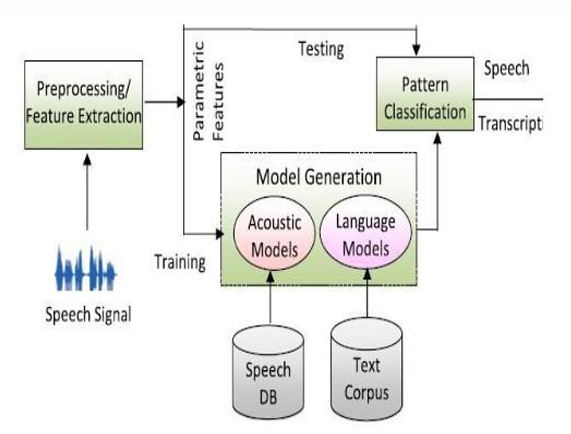
\includegraphics[width=0.7\linewidth]{imagens/stt.png}
     \label{fig:4}
     \footnote{\textbf{Fonte:} \cite{trivedi2018}}
\end{figure}

Alguns modelos que podem ser usados incluem o Whisper, da OpenAI \cite{radford2023}, e outros como o próprio Google Cloud Speech-to-Text e o wav2vec 2.0 \cite{Baevski2020}.

\subsection{Síntese de Voz: \textit{Text-to-Speech}}

A Síntese de Voz, conhecida como \textit{Text-to-Speech} (TTS), é uma tecnologia que converte texto escrito em fala artificial, permitindo que sistemas computacionais transformem conteúdos de texto em áudio. Segundo \citeonline{trivedi2018}, essa tecnologia tem sido amplamente utilizada em diversas aplicações, como assistentes virtuais, leitores de tela para acessibilidade e sistemas de navegação. O objetivo do TTS é transformar texto em um áudio inteligível e natural, aproximando-se ao máximo da fala humana.

O fluxo realizado pelas aplicações que realizam a síntese de voz possui basicamente dois módulos principais. De acordo com \citeonline{Dutoit1997}, são eles o módulo de Processamento de Linguagem Natural (NLP, do inglês Natural Language Processing) e o módulo de Processamento de Sinal Digital (DSP, do inglês Digital Signal Processing). \citeonline{Dutoit1997} explica que, de forma bem parecida com a fala humana:

\begin{citacao}
    …ela compreende um módulo de Processamento de Linguagem Natural (NLP), capaz de produzir uma transcrição fonética do texto lido, juntamente com a entonação e o ritmo desejados (frequentemente denominado como prosódia), e um módulo de Processamento de Sinal Digital (DSP), que transforma a informação simbólica que recebe em fala.
\end{citacao}

Na Figura \ref{fig:5}, pode-se perceber mais facilmente como o diagrama do sistema TTS processa as informações, primeiramente com um módulo de NLP, transcrevendo foneticamente o texto lido e, posteriormente, o texto é submetido ao módulo de DSP, que realiza a transformação do texto em fala.

\begin{figure}[!h]
     \caption{Exemplo simples do funcionamento do TTS}
     \centering
     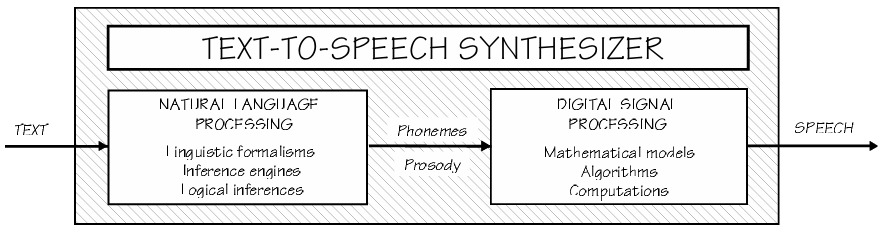
\includegraphics[width=0.7\linewidth]{imagens/tts.png}
     \label{fig:5}
     \footnote{\textbf{Fonte:} \cite{Dutoit1997}}
\end{figure}

Assim, embora a estrutura tradicional de sistemas TTS, baseada nos módulos de NLP e DSP, ainda seja amplamente utilizada, modelos mais modernos adotam arquiteturas aprimoradas para superar limitações de desempenho e qualidade da fala. Segundo \citeonline{popov2021}, as abordagens atuais incorporam técnicas de modelagem difusional probabilística, como o modelo Grad-TTS, que emprega um decodificador baseado em score para transformar gradualmente o ruído em mel-espectrogramas alinhados ao texto de entrada, utilizando o algoritmo de Monotonic Alignment Search (MAS) para aprimorar a correspondência entre texto e áudio. Essa abordagem permite um controle explícito do equilíbrio entre qualidade da síntese e velocidade de inferência, representando um avanço significativo sobre os métodos tradicionais baseados em atenção, como o Tacotron2.

Dessa forma, os sistemas modernos de TTS evoluíram para incorporar arquiteturas mais robustas, capazes de fornecer fala sintetizada com maior naturalidade e precisão, ao mesmo tempo em que reduzem os erros de pronúncia e aumentam a eficiência computacional.
\chapter{Metodologia}  \label{cap:03}

Este trabalho caracteriza-se como uma pesquisa aplicada de natureza experimental. Define-se como aplicada pois aborda um problema prático concreto - a carência de aplicativos capazes de descrever ambientes para pessoas com deficiência visual em tempo real — e busca, simultaneamente, promover a inclusão desse grupo minoritário no uso de IA. Já seu caráter experimental advém do desenvolvimento de um protótipo e da comparação de diferentes modelos de IA para a tarefa de descrição de imagens.

No que se refere à abordagem metodológica, há uma componente quantitativa, evidenciada na coleta de métricas (por exemplo, medição de latência e análise das descrições por meio de indicadores específicos) e na comparação estatística dos resultados entre os modelos. Em paralelo, há aspectos qualitativos na avaliação da coerência das legendas geradas, embora, nesta etapa, os testes tenham sido realizados apenas internamente pelo autor.

\section{Ferramentas e Tecnologias}

Nesta seção, descrevem-se os recursos de \textit{hardware}, \textit{software} e bibliotecas utilizados no desenvolvimento do aplicativo e na execução dos modelos de IA.

\subsection{\textit{Hardware} utilizado}

Para hospedar a API (Application Programming Interface) e oferecer suporte ao processamento dos modelos de LLM, utilizou-se um \textit{desktop} instalado no Instituto Federal de Mato Grosso do Sul (IFMS), Campus Três Lagoas. Esse computador apresenta as seguintes configurações:

\begin{itemize}
    \item \textbf{CPU:} 11th Gen Intel(R) Core(TM) i7-11700KF (8 núcleos físicos, 16 \textit{threads}, até 5,0 GHz)
    \item \textbf{GPU:} NVIDIA GeForce RTX 3070 (8 GiB de memória VRAM), Driver 550.107.02, suporte a CUDA 12.4
    \item \textbf{Memória:} 32 GiB DDR4
    \item \textbf{Armazenamento:} 1 TiB em SSD NVMe + RAID 5 (2,27 TiB) para armazenamento de dados
    \item \textbf{Sistema Operacional:} Debian GNU/Linux 12 (Bookworm), Kernel 6.1.0-13-amd64
\end{itemize}

Embora seja um ambiente favorável a testes com modelos de IA, a memória de 8 GiB da GPU pode se tornar um fator limitante para modelos de linguagem maiores. Além disso, a execução via CPU, caso o modelo exceda a capacidade da GPU, tende a prejudicar a latência das requisições. Nesse sentido, reforça-se o caráter experimental do desenvolvimento, pois a viabilidade plena da solução em cenários mais complexos depende de recursos computacionais adicionais, além de técnicas de otimização de modelos, como a quantização, que serão utilizadas para melhorar a performance neste projeto.

A quantização se apresenta como uma solução essencial para reduzir o consumo de memória e melhorar a eficiência computacional de redes neurais, tornando possível a execução de modelos de grande porte em dispositivos com recursos limitados. De acordo com \citeonline{Wei2024}, essa técnica permite diminuir a largura de banda necessária para a transmissão de dados e otimiza a velocidade de inferência sem comprometer significativamente a precisão dos modelos.

De forma geral, seguindo a definição de \citeonline{Wei2024}, a quantização é o processo de conversão de redes neurais que utilizam números de ponto flutuante em redes neurais de largura de bits reduzida, geralmente inteiras, com o objetivo de minimizar o custo computacional e o consumo de energia, tornando viável a implantação de modelos em ambientes de computação de borda. Assim, ao adotar essa técnica, busca-se equilibrar desempenho e eficiência, permitindo a execução otimizada do modelo no \textit{hardware} disponível.

\subsection{Aplicativo \textit{mobile}}

Para o módulo de aplicativo, foram consideradas ferramentas que aliassem eficiência no desenvolvimento e aderência aos requisitos do projeto, sobretudo o de desenvolver uma solução multiplataforma (Android e iOS). A partir dessas premissas, optou-se pelo \textit{framework} Flutter, conhecido, principalmente, por sua produtividade, trazendo agilidade na construção do aplicativo tanto para iOS como para Android, e uma comunidade ativa, onde é disponibilizado um amplo conjunto de pacotes e bibliotecas que aceleram o desenvolvimento.

Dentre as bibliotecas utilizadas, destacam-se:

\begin{itemize}
    \item \textbf{\texttt{flutter\_tts}:} Responsável pela conversão de texto em fala (TTS).
    \item \textbf{\texttt{flutter\_sound}:} Permite a gravação de áudios, viabilizando a utilização do áudio para o usuário questionar o que está na sua frente.
    \item \textbf{\texttt{camera}:} Facilita o acesso à câmera do dispositivo, para captura de imagens.
    \item \textbf{\texttt{http}:} Simplifica a realização de requisições REST à API desenvolvida em Python.
\end{itemize}

A escolha do Flutter visa garantir acessibilidade e praticidade no desenvolvimento, além de oferecer pacotes para a conexão direta com o \textit{hardware}, algo que é essencial para o projeto e garantia da usabilidade pelo usuário nos diferentes sistemas operacionais móveis.

\subsection{API}

O módulo da API foi implementado com o intuito de receber as imagens e os áudios do aplicativo, processá-los por meio de modelos de IA e retornar as descrições geradas, para, posteriormente, serem reproduzidos pelo aplicativo novamente. Para isso, adotou-se a linguagem Python, na versão 3.11.2, devido à ampla disponibilidade de bibliotecas de \textit{Machine Learning} e à gama de suporte existente da comunidade. Além do exposto, aliado à grande comunidade de desenvolvedores em Python, soma-se a disponibilidade de \textit{frameworks}, que visa trazer eficiência para o desenvolvimento. Desta forma, para este trabalho foi utilizado o \textit{framework web} FastAPI, que simplifica a criação de \textit{endpoints} REST (Representational State Transfer API) e facilita a escalabilidade e manutenção do servidor.

No servidor, os modelos ficam salvos, e o aplicativo se comunica com eles por meio da API hospedada no próprio servidor. A API fica responsável por:

\begin{enumerate}
    \item Receber a imagem e o áudio vindos do aplicativo Flutter, via requisição HTTP.
    \item Transcrição do áudio recebido com o questionamento sobre o ambiente.
    \item Pré-processar a imagem (por exemplo, redimensionar, normalizar).
    \item Executar o modelo de LLM escolhido para gerar a descrição da imagem.
    \item Retornar o texto descritivo ao aplicativo, que então o converte em áudio por meio do \texttt{flutter\_tts}.
\end{enumerate}

A flexibilidade do Python e do FastAPI permite alternar rapidamente entre diferentes modelos de IA, facilitando o processo de \textit{benchmark} e garantindo a modularidade do sistema.

\subsection{Modelos de IA}

Para a tarefa de descrição de imagens, este trabalho faz uso de três LLMs de código aberto disponíveis no Hugging Face:

\begin{itemize}
    \item \textbf{\texttt{Qwen/Qwen2.5-VL-7B-Instruct}:} possui um tamanho de 7 bilhões de parâmetros. Isto balança bom desempenho em legendagem de imagens com latência moderada, podendo ser executado em GPU de 8 GiB.
    \item \textbf{\texttt{llava-hf/llava-v1.6-mistral-7b-hf}:} também com 7 bilhões de parâmetros. Tem se destacado em instruções multimodais e apresenta boa relação entre desempenho e consumo de recursos, além de sua arquitetura ser utilizada por diversos outros modelos.
    \item \textbf{\texttt{meta-llama/Llama-3.2-11B-Vision-Instruct}:} possui 11 bilhões de parâmetros. Capaz de descrever melhor as imagens, porém mais exigente em termos de memória e processamento, podendo afetar a latência e o consumo de GPU.
\end{itemize}

Já para o processamento do áudio, ou seja, o processo de STT, também foi utilizado um modelo do Hugging Face, mais especificamente o modelo \texttt{openai/whisper-small} \cite{radford2023}. Este modelo foi escolhido por conta da sua grande capacidade de fazer transcrições, mesmo sendo um modelo pequeno, o que economiza recursos do \textit{desktop} disponível.

Cada modelo é carregado em Python por meio das bibliotecas Transformers (Hugging Face) e PyTorch, permitindo alternar rapidamente entre as opções durante os testes. A motivação para essa variedade de modelos é evidenciar as vantagens e limitações de cada abordagem em termos de acurácia descritiva e velocidade de processamento, reforçando o caráter experimental do desenvolvimento.

Os modelos foram escolhidos de forma empírica, visando principalmente garantir que seria possível a execução na máquina disponibilizada. Outros modelos também poderiam ser testados, porém, para efeitos de prototipagem, foram selecionados os três supracitados.

\subsection{TTS}

O processo do TTS é imprescindível para tornar as descrições de ambiente acessíveis a pessoas com deficiência visual utilizando IA. Neste projeto, optou-se por executar o TTS diretamente no aplicativo \textit{mobile}, visando, principalmente, a redução da latência e dos dados trafegados via rede, assegurando, desta forma, que o usuário possa receber a mensagem mesmo em conexões mais instáveis.

Para isso, empregou-se a biblioteca \texttt{flutter\_tts}, amplamente utilizada em aplicações Flutter. Ela foi escolhida tanto por sua integração simples em aplicativos como também pelas opções de customização, que podem facilmente ser ajustadas. 

Assim, o processo de descrição ocorre em duas etapas: (1) o servidor gera o texto com a descrição da imagem capturada e (2) o aplicativo recebe essa legenda e chama a função de TTS para sintetizar a fala em tempo real.

\section{Arquitetura do Sistema}

A fim de integrar de forma coerente o aplicativo \textit{mobile} e o servidor que hospeda os modelos de IA, projetou-se uma arquitetura orientada a serviços, conforme ilustrado na Figura \ref{fig:6}. Nela, o fluxo de dados segue as seguintes etapas: (1) captura de imagem e do áudio por meio de um gatilho, que foi definido como o toque na tela, (2) realização da requisição à API enviando a imagem e o áudio capturados, (3) o áudio é convertido em texto, por meio do modelo STT, (4) processamento pelo modelo LLM, (5) retorno do texto descritivo ao aplicativo e (6) conversão desse texto em fala (TTS).

\begin{figure}[!ht]
     \caption{Arquitetura do sistema (alto-nível)}
     \centering
     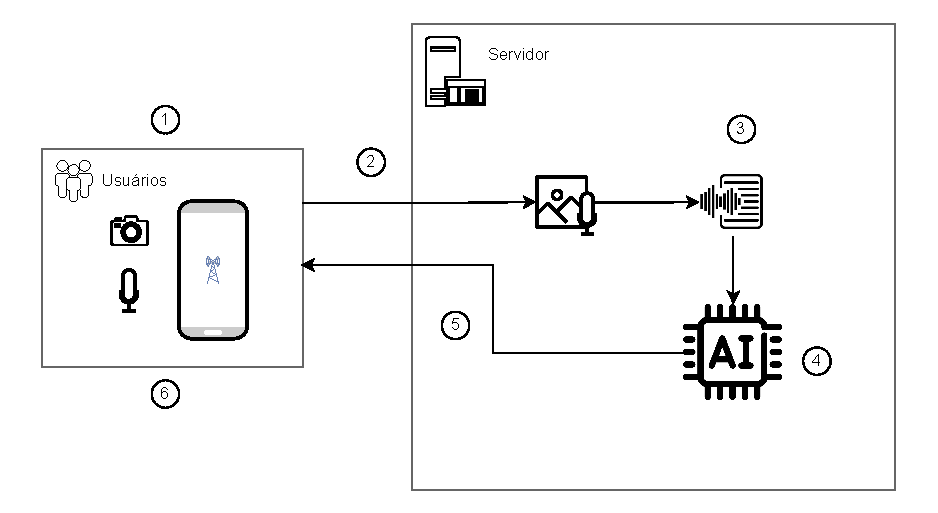
\includegraphics[width=0.7\linewidth]{imagens/architeture-tcc.drawio.pdf}
     \label{fig:6}
     \footnote{\textbf{Fonte:} Elaborado pelo Autor (2025)}
\end{figure}

Observa-se, portanto, que a arquitetura proposta facilita a interação entre Aplicativo (Flutter), API (FastAPI) e Modelos de IA para a descrição de imagens e o processamento de áudio. A abordagem orientada a serviços permite escalabilidade e manutenção simplificadas, já que cada componente (captura da imagem, conversão de áudio em texto, geração de legenda via LLM e TTS) pode ser atualizado ou substituído independentemente, sem impactar as demais partes do sistema.

\begin{figure}[!h]
     \caption{Diagrama de Sequência}
     \centering
     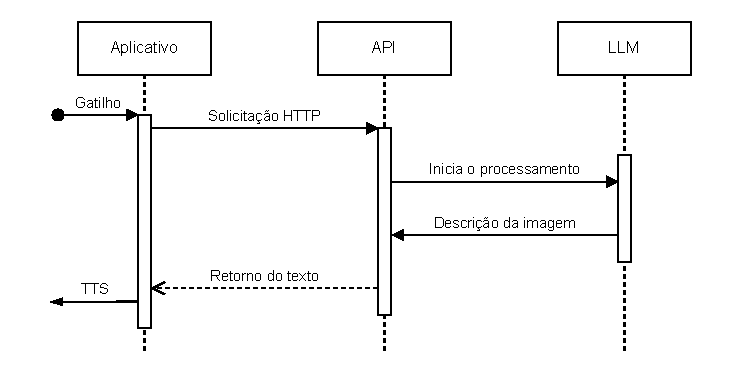
\includegraphics[width=0.7\linewidth]{imagens/diagrama_sequencia.drawio.pdf}
     \label{fig:7}
     \footnote{\textbf{Fonte:} Elaborado pelo Autor (2025)}
\end{figure}

A Figura \ref{fig:7} complementa a visão geral apresentada na Figura \ref{fig:6} ao detalhar, em formato de diagrama de sequência, as trocas de mensagens e o encadeamento temporal das chamadas entre o aplicativo, servidor e o LLM. Dessa forma, fica evidenciado que o processo se inicia na captura de multimídia (imagem e áudio), passa pelo envio dos dados à API e pela execução dos modelos de STT e LLM, e retorna ao aplicativo na forma de texto, convertido em áudio pelo TTS. Esse fluxo modular possibilita, ainda, testes de \textit{benchmark} para avaliar diferentes configurações ou modelos de IA sem a necessidade de alterações estruturais no aplicativo móvel.

\section{Procedimentos de Desenvolvimento}

Nesta seção, descreve-se o passo a passo para o desenvolvimento do protótipo, abrangendo desde a captura da imagem e a gravação de áudio no aplicativo Flutter até o retorno da descrição em áudio, com ênfase no processo de modularização que viabiliza a comparação de diferentes modelos de IA. O detalhamento segue a lógica de comunicação entre os módulos, já ilustrada na Figura \ref{fig:7}.

\subsection{Aplicativo}

Conforme destacado em seções anteriores, a escolha do \textit{framework} Flutter para o desenvolvimento do aplicativo se deve à necessidade de atender múltiplas plataformas (Android e iOS) de forma eficiente. Antes de iniciar a construção efetiva do aplicativo, procedeu-se a um planejamento detalhado para definir o melhor gatilho de captura, levando em conta que processos contínuos, disparados automaticamente, trariam um custo elevado tanto em termos de arquitetura quanto de processamento.

Inicialmente, cogitou-se o uso dos botões de volume como disparadores, mas concluiu-se que tal solução interferiria na alteração do volume do dispositivo, comprometendo a usabilidade. Por fim, optou-se pelo toque na tela, em que um primeiro toque inicia a gravação de áudio e a captura da imagem, e um segundo toque encerra a gravação, sinalizando que todo o material coletado (imagem e áudio) deve ser enviado à API.

Em termos de \textit{design} e construção de telas, decidiu-se que, dada a natureza do aplicativo — voltado para pessoas com deficiência visual —, uma interface minimalista seria mais adequada. Nesse sentido, retoma-se o argumento de \citeonline{Torres2002}, segundo o qual a usabilidade para esse público requer interfaces enxutas e objetivas. Assim, a aplicação conta basicamente com uma única tela, exibindo a câmera em tempo real. O usuário toca na tela para iniciar a coleta de dados (imagem e áudio) e, ao tocar novamente, finaliza o processo e envia todo o conteúdo ao servidor. As instruções de uso do aplicativo serão dadas por meio da biblioteca \texttt{flutter\_tts}, que permitirá ao usuário, quando iniciar o aplicativo, receber uma mensagem explicativa sobre como se dará o uso.

Após a captura da imagem e do áudio, e o posterior envio desse conteúdo ao servidor, o aplicativo aguarda a resposta do modelo de IA. Uma vez que o texto descritivo é recebido, o Flutter aciona a biblioteca \texttt{flutter\_tts} novamente, que converte a legenda retornada em fala. Esse processo de síntese de voz local evita atrasos adicionais na comunicação com o servidor, tornando a experiência mais fluida. Dessa forma, o usuário com deficiência visual pode ouvir a descrição do ambiente ou objeto em tempo real, fechando o ciclo de interação.

Para a implementação, empregaram-se as seguintes bibliotecas do ecossistema Flutter:

\begin{itemize}
    \item \textbf{\texttt{camera}:} Acesso à câmera do dispositivo, capturando a imagem a ser processada.
    \item \textbf{\texttt{flutter\_sound}:} Captação de áudio, viabilizando a gravação pelo microfone do dispositivo.
    \item \textbf{\texttt{http}:} Envio dos dados (imagem e áudio) ao servidor, por meio de requisições HTTP.
    \item \textbf{\texttt{flutter\_tts}:} Conversão do texto em áudio, permitindo que o usuário receba a descrição final por meio de fala sintetizada.
\end{itemize}

Assim, o aplicativo concentra as duas pontas essenciais do sistema: a coleta (imagem e áudio) e a reprodução da descrição (TTS), enquanto o processamento de IA (incluindo o STT e a descrição da imagem) permanece centralizado no servidor.

\subsection{API}

Assim como no desenvolvimento do aplicativo, a API foi concebida de forma modular e objetiva, buscando equilibrar simplicidade de arquitetura e possibilidade de troca de modelos de IA. Para isso, optou-se pela linguagem Python em conjunto com o FastAPI, tendo em vista a praticidade na criação de endpoints REST e a integração direta com bibliotecas de \textit{Machine Learning}. Embora inicialmente se tenha cogitado a adoção de contêineres Docker para isolar o ambiente, as restrições relacionadas ao uso de GPU acabaram direcionando a escolha para a execução direta via \texttt{uvicorn}, reduzindo potenciais problemas de compatibilidade.

Em termos de fluxo, a API cumpre o papel de receber a imagem e o áudio enviados pelo aplicativo, processá-los usando modelos de IA e retornar a descrição gerada. Para isso, a inicialização da API ocorre em um arquivo principal, no qual são instanciadas as classes responsáveis pelo processamento de áudio (transcrição) e pela descrição de imagens. Durante a fase de inicialização do serviço, esse arquivo principal carrega e armazena as instâncias desses componentes, tornando-as disponíveis em toda a aplicação. Dessa forma, sempre que um \textit{endpoint} for acionado, o sistema já dispõe de objetos especializados prontos para lidar com a inferência em IA.

Com a estrutura básica definida, um arquivo de rotas agrega as funções de processamento que recebem dados enviados pelo aplicativo (imagem e áudio) e orquestram o fluxo de tratamento, centralizando-se no \textit{endpoint} principal, responsável pelo fluxo, que foi denominado de \texttt{/analyze-image-audio-query}, facilitando a compreensão do objetivo do mesmo. Nesse fluxo, o áudio pode ser transcrito por uma classe de processamento específica, enquanto a imagem passa por um pré-processamento, que realiza o redimensionamento da imagem por restrições de memória, antes de ser submetida ao LLM para geração da descrição. Ao término dessas etapas, a rota retorna um objeto JSON que reúne tanto o texto transcrito do áudio quanto a descrição do conteúdo visual, cabendo ao aplicativo converter esses resultados em fala ou exibir de outra forma.

Para viabilizar a troca de modelos sem sobrecarregar o desenvolvedor, adotou-se uma lógica de configuração na qual, ao iniciar o serviço, define-se o modelo a ser carregado, esse carregamento se dá por meio do nome do modelo, conforme já supracitado. Esse modelo permanece em memória, priorizando o uso da GPU e, caso não haja espaço suficiente, se divide entre GPU e CPU, afetando a latência da resposta do modelo, o que melhora o desempenho das requisições subsequentes. Esse mecanismo de modularização permite rapidamente substituir o modelo em uso, facilitando experimentos e \textit{benchmarks}. Além disso, classes específicas cuidam do áudio e da imagem, isolando responsabilidades e garantindo que cada parte do sistema possa ser aprimorada ou substituída com o mínimo de impacto no restante da aplicação.

Em suma, a API executa o processamento pesado de IA, recebendo o material capturado pelo aplicativo e produzindo descrições para as imagens. Enquanto o aplicativo concentra a captura (imagem e áudio) e a reprodução (TTS), a API lida com as tarefas de computação intensiva, mantendo o fluxo geral simples e modular. Essa separação de papéis, aliada à flexibilidade na escolha e substituição de modelos, faz com que o sistema seja altamente adaptável às futuras necessidades de acessibilidade e evolução tecnológica.

\subsection{LLM}

Dando continuidade ao fluxo de desenvolvimento, a carga e o gerenciamento dos modelos de linguagem são etapas fundamentais para viabilizar o processamento de imagens no servidor. Assim como ocorreu nos módulos de Aplicativo e API, buscou-se adotar uma abordagem modular, onde cada aspecto do carregamento e da execução dos LLMs fosse isolado e configurável, facilitando alterações e \textit{benchmarks} futuros.

Em linhas gerais, o carregamento dos modelos ocorre no arquivo responsável pelo processamento de imagem, por meio de uma classe que inicializa e gerencia diferentes LLMs. Ainda na fase de inicialização do servidor, o código verifica se a GPU está disponível, isto é, se o dispositivo possui suporte a CUDA, para então definir parâmetros como \texttt{torch\_dtype}, além de um mapeamento de dispositivos, o que possibilita distribuir partes do modelo entre CPU e GPU caso a memória da placa não seja suficiente para comportar todo o modelo de uma só vez.

\subsubsection{Quantização e Otimização da Memória}

Dado que a quantidade de memória em GPU não era tão alta e a expansão era inviável no momento, foi empregada a quantização via \texttt{BitsAndBytesConfig}, implementada via Transformers do Hugging Face. Quando a execução detecta que há uma GPU disponível, o código habilita o carregamento em \texttt{4-bit}, com a intenção de reduzir o espaço requerido pelos pesos do modelo. Nesse processo, configurações como \texttt{bnb\_4bit\_quant\_type} e \texttt{bnb\_4bit\_compute\_dtype} ajudam a manter um equilíbrio entre desempenho e economia de memória. Essa quantização também permite \textit{offload} de partes do modelo para CPU quando necessário, evitando estouros de memória na GPU.

Outra técnica que visa garantir a utilização eficiente dos recursos disponíveis é o mapeamento de dispositivos, que ocorre de forma automática, graças aos recursos fornecidos pela biblioteca Transformers, que detectam quanta memória está livre na GPU e alocam dinamicamente os \textit{layers} dos modelos em diferentes locais (GPU/CPU) conforme a necessidade. Dessa forma, modelos que tradicionalmente seriam muito grandes para caber na GPU, como o LLaMa 3.2, podem ser parcialmente alocados na memória de vídeo, enquanto outras partes permanecem na CPU, garantindo que o sistema não entre em colapso por falta de espaço.

\subsubsection{Fluxo de Carregamento}

Para facilitar e seguir os padrões de utilização da biblioteca Transformers, o seguinte fluxo foi aplicado:

\begin{enumerate}
    \item Antes de efetuar qualquer \textit{download} ou instanciação, o sistema verifica se o modelo requisitado já foi carregado anteriormente. Caso afirmativo, apenas retorna a instância armazenada em memória.
    \item Se o \textit{hardware} de destino tiver GPU disponível, aplica-se a quantização, valendo-se do \texttt{BitsAndBytesConfig} configurando o \texttt{load\_in\_4bit} e os parâmetros de \texttt{quant\_type}. Quando a execução ocorre apenas em CPU, carrega-se o modelo sem quantização ou com configurações específicas para esse cenário.
    \item Como este trabalho utiliza 3 modelos diferentes, a cada alteração de modelo são chamados métodos específicos para cada um deles, garantindo, desta forma, que cada um deles tenha a capacidade de execução adequada conforme sua configuração. Para modelos grandes, como o LLaMa, ainda pode-se definir parâmetros como \texttt{max\_memory} para indicar à biblioteca quanta memória a GPU pode usar.
    \item Uma vez carregado, o modelo é armazenado em um dicionário de instâncias, evitando duplicações. As próximas requisições podem então aproveitar o mesmo objeto, reduzindo a latência na fase de inferência.
\end{enumerate}

Em resumo, a adoção de quantização e mapeamento dinâmico de dispositivos configura uma estratégia essencial para lidar com modelos robustos em ambientes com recursos limitados. Dessa forma, mesmo com GPUs relativamente modestas, pode ser possível a condução de experimentos de \textit{image captioning} usando LLMs de última geração, mantendo a latência sob controle e promovendo a escalabilidade do sistema.

\section{Estratégia de Benchmark}

A fim de comparar objetivamente os modelos de IA adotados, estabeleceu-se uma estratégia de \textit{benchmark} baseada em critérios de seleção, métricas de comparação e cenários de teste que refletem diferentes graus de complexidade. Por meio dessa abordagem, espera-se avaliar tanto o desempenho técnico, em termos de latência e qualidade de legendas, quanto a adaptabilidade dos modelos em situações reais de uso.

\subsection{Seleção de Modelos}

A escolha dos modelos considerou fatores como tamanho, qualidade prévia e compatibilidade com o \textit{hardware} disponível, uma vez que o número de parâmetros impacta diretamente no tempo de execução e no consumo de memória da GPU. Aspectos como licenças de uso para fins de pesquisa e a documentação associada a cada modelo também foram avaliados, visando garantir tanto a legalidade do experimento quanto um desenvolvimento mais ágil.

Com base nesses critérios, selecionaram-se três arquiteturas principais: \texttt{Qwen2.5-VL-7B-Instruct}, \texttt{llava-v1.6-mistral-7b-hf} e \texttt{Llama-3.2-11B-Vision-Instruct}. Os dois primeiros, ambos em torno de 7 bilhões de parâmetros, apresentam consumo de recursos mais modesto, o que tende a resultar em menor latência e maior compatibilidade com GPUs de médio porte. Já o terceiro, com 11 bilhões de parâmetros, pode oferecer descrições mais abrangentes, porém a um custo computacional mais elevado, exigindo maior memória de vídeo e poder de processamento. 

Em todos os casos, as licenças permissivas e a documentação disponível contribuíram para facilitar a integração e a eventual adaptação no contexto de pesquisa, assegurando, ao mesmo tempo, suporte ativo e referências práticas para a implementação.

\subsection{Métricas de Comparação}

Para definir qual dos modelos selecionados será efetivamente adotado no protótipo final, planeja-se aplicar um \textit{benchmark} que submeterá cada um a uma série de testes com imagens extraídas de um \textit{dataset} público, com as imagens já rotuladas (no caso deste trabalho, utilizou-se o coco-captions-pt-br \cite{bromonschenkel2024cocopt}). A avaliação considerará tanto indicadores quantitativos quanto qualitativos, a fim de mensurar de maneira abrangente o desempenho de cada arquitetura.

Do ponto de vista quantitativo, a latência desponta como métrica essencial, pois indica o tempo transcorrido entre o envio de uma imagem e a obtenção da legenda final. Considerando que o aplicativo visa auxiliar pessoas com deficiência visual em tempo real, latências elevadas prejudicam a experiência do usuário ao retardar a entrega da descrição. Para conferir robustez estatística aos resultados, cada modelo será testado repetidamente, registrando-se a média, mediana e o desvio padrão da sua latência de resposta.

No tocante à qualidade textual, adotar-se-á um conjunto de métricas que inclui BERTScore \cite{Zhang2020:} e ROUGE-L \cite{lin-2004-rouge}. O BERTScore, baseado em \textit{embeddings} de \textit{tokens}, mede a similaridade semântica entre a descrição gerada e uma legenda de referência, indo além de simples contagens de n-gramas. Segundo \citeonline{Zhang2020:}, para medir similaridade textual, o BERTScore utiliza \textit{embeddings} contextualizados de palavras, comparando cada \textit{token} da sequência gerada com os \textit{tokens} da referência por meio da similaridade do cosseno entre seus vetores de representação. Isso permite que o método capture sinônimos e estruturas semânticas mais flexíveis, superando as limitações de métricas baseadas apenas em correspondência exata de palavras.

Por outro lado, o ROUGE-L avalia a maior sequência comum de palavras (\textit{Longest Common Subsequence}), proporcionando uma análise léxica da sobreposição de conteúdo entre o texto produzido e o de referência. De acordo com \citeonline{lin-2004-rouge}, o ROUGE-L mede o comprimento da subsequência comum mais longa entre o texto candidato e a referência, atribuindo uma pontuação maior a textos que preservam a estrutura e ordem das palavras. Isso o torna uma métrica útil para avaliar se a estrutura da resposta gerada mantém coerência com o texto de referência. Juntas, essas métricas equilibram uma perspectiva semântica (BERTScore) e uma aproximação lexical (ROUGE-L), oferecendo um panorama sólido sobre a fidelidade das legendas.

Em caráter adicional, será realizada uma avaliação manual para verificar a coerência das descrições. Embora não estejam previstos testes extensivos com voluntários neste estágio, o escrutínio por parte do autor e do orientador permitirá identificar possíveis falhas severas, como omissões importantes ou a “invenção” de objetos inexistentes. A soma das análises quantitativas e qualitativas viabiliza uma escolha mais criteriosa do modelo a ser integrado ao aplicativo final, assegurando que o sistema atenda às necessidades de acessibilidade e desempenho simultaneamente.

\subsection{Cenários de Teste}

Para garantir que as medições realizadas reflitam condições diversas de uso, decidiu-se empregar dois tipos de abordagens na escolha das imagens. Primeiramente, definiu-se a adoção do \textit{coco-captions-pt-br} \cite{bromonschenkel2024cocopt}, uma versão adaptada para o português do Brasil do conhecido conjunto de dados COCO (\textit{Common Objects in Context}). Esse \textit{dataset} reúne um amplo espectro de cenários e objetos, indo de imagens simples (um ou poucos objetos isolados) até cenas mais complexas e sobrecarregadas de elementos, o que favorece uma avaliação robusta das capacidades de cada modelo. A variedade presente no \textit{coco-captions-pt-br} possibilita aferir como as redes lidam com distintos níveis de complexidade, bem como a coerência das descrições fornecidas em situações mais desafiadoras.

Além disso, serão realizados testes práticos pelo autor em cenários típicos do cotidiano, como ruas, jardins e ambientes internos (salas de aula, áreas externas e laboratórios do ambiente acadêmico). Pretende-se, assim, verificar o desempenho dos modelos em condições de iluminação variada e em situações onde objetos possam se sobrepor ou aparecer em planos de fundo confusos. Dessa forma, tornam-se evidentes possíveis limitações, como a dificuldade de reconhecer pessoas em ambientes pouco iluminados, a omissão de detalhes importantes ou a “invenção” de elementos não existentes na imagem. Em conjunto, esse arranjo de testes, incluindo tanto um conjunto de dados público e sistematizado quanto exemplos reais do dia a dia, fornece subsídios mais completos para avaliar o quão eficazes os modelos são na tarefa de gerar descrições confiáveis, fator essencial na proposta de auxiliar pessoas com deficiência visual em tempo real.


% A metodologia consiste num conjunto de etapas ordenadamente dispostas a serem executadas e que tenham por finalidade a investigação de fenômenos para a obtenção de conhecimentos. Basicamente, compõe-se de etapas dispostas de forma sistemática, obedecendo a uma forma sequencial. 

% Sendo assim, para a elaboração de um Trabalho de Pesquisa em Tecnologia da Informação, é preciso responder detalhadamente as seguintes questões:\\

% \textbf{Como se procederá a pesquisa?}

% % enumerate é um comando que insere listas numeradas
% \begin{enumerate}
%     \item Qual será o tema da sua pesquisa? 
%     \item Qual o espaço (local ou área) delimitado da pesquisa? 
%     \item Qual é o pretende resolver?
%     \item Qual será o tipo da sua pesquisa? Desenvolvimento de Software ou Pesquisa Bibliográfica?
%     \item Se for realizar pesquisa Bibliográfica, qual será sua área de estudo? Que autores pretende abordar?
%     \item Pretende realizar questionários ou entrevistas com pessoas da área?
%     \item Se a pesquisa for de desenvolvimento de software, como será feita a análise de requisitos? Quem será consultado? 
%     \item Como será construída a documentação do Sistema?
%     \item Quais serão as tecnologias utilizadas para a documentação, desenvolvimento e testes de software?
%     \item Como o sistema será construído?
%     \item Como será implementado o sistema?
%     \item Se for realizar testes de software, qual método pretende adotar?
% \end{enumerate}

\chapter{Resultados e Discussões} \label{cap:04}

Esta seção apresenta a análise aprofundada dos experimentos realizados durante o desenvolvimento do protótipo. Foram empregados testes quantitativos e qualitativos com o objetivo de comparar três modelos de IA para a tarefa de descrição de imagens. Para tanto, o \textit{benchmark} abrangeu métricas de latência, qualidade textual (utilizando BERTScore e ROUGE-L) e testes manuais, de forma a avaliar a coerência e a utilidade das descrições geradas. Em seguida, realiza-se uma análise crítica dos resultados, destacando os \textit{trade-offs} encontrados, e, finalmente, são discutidas as principais limitações do sistema desenvolvido.

\section{Resultados do \textit{Benchmark}}

Nesta seção, são apresentados e discutidos os resultados dos testes de \textit{benchmark} desenvolvidos para comparar os modelos escolhidos, com o objetivo de definir qual deles é o mais adequado para a construção do protótipo assistivo. Os experimentos quantitativos foram conduzidos utilizando o \textit{dataset} público \texttt{coco-captions-pt-br} \cite{bromonschenkel2024cocopt}, que reúne imagens de diversos cenários – desde composições simples até ambientes com alta complexidade visual. Para cada modelo, foram coletadas as seguintes métricas:

\begin{itemize}
    \item \textbf{Latência:} Tempo médio, mediano e desvio padrão (em segundos) medindo o intervalo entre o envio da imagem para a API e o recebimento da descrição.
    \item \textbf{BERTScore:} Métrica que avalia a similaridade semântica entre a descrição gerada e as legendas de referência. A pontuação varia de 0 a 1, onde 0 indica nenhuma similaridade semântica entre os textos e 1 representa uma correspondência perfeita, considerando a proximidade de significado entre as palavras e suas representações contextuais.
    \item \textbf{ROUGE-L:} Índice que analisa a sobreposição lexical, mensurando a maior sequência comum de palavras entre o texto gerado e o de referência. Seu valor também varia de 0 a 1, onde 0 significa que não há palavras em comum entre os textos e 1 indica que o texto gerado é idêntico à referência em termos de estrutura lexical.

\end{itemize}

Essas métricas permitem uma avaliação integrada, capturando tanto a qualidade textual das descrições quanto o desempenho em termos de velocidade de processamento de cada modelo. 

Na Tabela \ref{tab:2} são apresentados os resultados quantitativos do \textit{benchmark}.

\begin{table}[!ht]
\centering
\caption{Desempenho médio dos modelos em termos de latência e qualidade textual}
\label{tab:2}
\resizebox{\columnwidth}{!}{%
\begin{tabular}{@{}
>{\columncolor[HTML]{FFFFFF}}l 
>{\columncolor[HTML]{FFFFFF}}l 
>{\columncolor[HTML]{FFFFFF}}l 
>{\columncolor[HTML]{FFFFFF}}l 
>{\columncolor[HTML]{FFFFFF}}l 
>{\columncolor[HTML]{FFFFFF}}l @{}}
\toprule
\multicolumn{1}{c}{\cellcolor[HTML]{FFFFFF}\textbf{Modelo}} &
  \multicolumn{1}{c}{\cellcolor[HTML]{FFFFFF}\textbf{BERTScore}} &
  \multicolumn{1}{c}{\cellcolor[HTML]{FFFFFF}\textbf{ROUGE-L}} &
  \multicolumn{1}{c}{\cellcolor[HTML]{FFFFFF}\textbf{Lat. Média (s)}} &
  \multicolumn{1}{c}{\cellcolor[HTML]{FFFFFF}\textbf{Lat. Mediana (s)}} &
  \multicolumn{1}{c}{\cellcolor[HTML]{FFFFFF}\textbf{Lat. Desvio Padrão (s)}} \\ \midrule
\texttt{llava-v1.6-mistral-7b-hf}      & 0,6840 & 0,1348 & 6,51    & 5,83    & 3,24        \\
\texttt{Qwen2.5-VL-7B-Instruct}        & 0,6966 & 0,1489 & 3,56    & 3,45    & 0,80        \\
\texttt{Llama-3.2-11B-Vision-Instruct} & 0,6770 & 0,1099 & 35,3967 & 31,1688 & 16,84627806
\end{tabular}%
}
\end{table}

Os dados obtidos evidenciam que o \texttt{Qwen2.5-VL-7B-Instruct} apresenta um desempenho superior no que diz respeito à latência, com uma média de 3,56 segundos, mediana de 3,45 segundos e um desvio padrão bastante baixo (0,80 s). Esse desempenho é crucial para aplicações em tempo real, onde a rapidez na entrega da descrição é essencial para a experiência do usuário final.

Em contrapartida, o modelo \texttt{llava-v1.6-mistral-7b-hf} apresentou uma latência média significativamente maior (6,51 s), com maiores variações nos tempos de resposta. Apesar de suas métricas de qualidade textual serem compatíveis, essa diferença de performance impacta negativamente sua viabilidade para aplicações em que o tempo de resposta é crítico.

Quanto ao \texttt{Llama-3.2-11B-Vision-Instruct,} devido ao seu tamanho e maior quantidade de parâmetros, surgiram desafios técnicos relacionados à capacidade da infraestrutura utilizada. Inicialmente, ao tentar rodar esse modelo utilizando a GPU por meio do Transformers do Hugging Face, os testes foram inviabilizados pelas limitações de memória da placa, até mesmo aplicando técnicas de otimização, como a quantização e a divisão do modelo entre GPU e CPU, em ambos os casos a memória era excedida e a execução era parada. Quando a execução foi realizada exclusivamente na CPU, o tempo de resposta ultrapassava 30 minutos, inviabilizando a aplicação prática do modelo. Para contornar esse obstáculo, optou-se por utilizar o Ollama, uma plataforma de código aberto que permite a execução de modelos de IA, principalmente LLMs, em hardware local \cite{bem2024}, que facilitou a integração e permitiu a realização dos testes. Embora o retorno das solicitações tenha sido obtido por meio do Ollama, a latência média permaneceu alta (35,4 segundos) e, apesar da qualidade textual apresentada ser boa, ela não superou a performance do \texttt{Qwen2.5-VL-7B-Instruct} e nem do \texttt{llava-v1.6-mistral-7b-hf}.

Outro aspecto a ser destacado refere-se ao teste exaustivo com 1000 imagens para todos os modelos. Durante esses testes, o modelo \texttt{Qwen2.5-VL-7B-Instruct} não conseguiu retornar a resposta para todas as requisições, sendo um resultado que se justifica pelo estresse imposto à GPU, evidenciando limitações na memória quando as solicitações são enviadas em sequência sem intervalos e ressaltando a importância de uma infraestrutura mais avançada para avanço nos desenvolvimentos. Entretanto, durante os testes manuais, realizados com um intervalo maior entre as solicitações, que seria o tempo normal de utilização do usuário, não foram observados erros ou falhas, demonstrando a robustez do modelo em condições operacionais normais.

\subsection{Análise Qualitativa com Imagem do \textit{dataset}}

Além das métricas quantitativas discutidas na Tabela \ref{tab:2}, realizou-se também uma avaliação qualitativa por meio de descrições geradas para duas imagens selecionadas do \textit{dataset}. Esse procedimento visa ilustrar a capacidade de cada modelo em identificar contextos, detalhes arquitetônicos ou de objetos, bem como avaliar a latência em situações próximas às de uso real. Ambas as imagens foram selecionadas no \textit{dataset} e avaliadas perante as descrições de cada um dos modelos.

Na Figura \ref{fig:8}, apresenta-se a St Pancras International Station, um edifício inaugurado em 1868, em Londres, que trata-se de um ponto turístico na cidade. A imagem foi utilizada para avaliar a precisão e a riqueza de detalhes das descrições, já que apresenta elementos arquitetônicos marcantes e céu parcialmente nublado.

\begin{figure}[!ht]
     \caption{Fotografia da estação ferroviária de St Pancras}
     \centering
     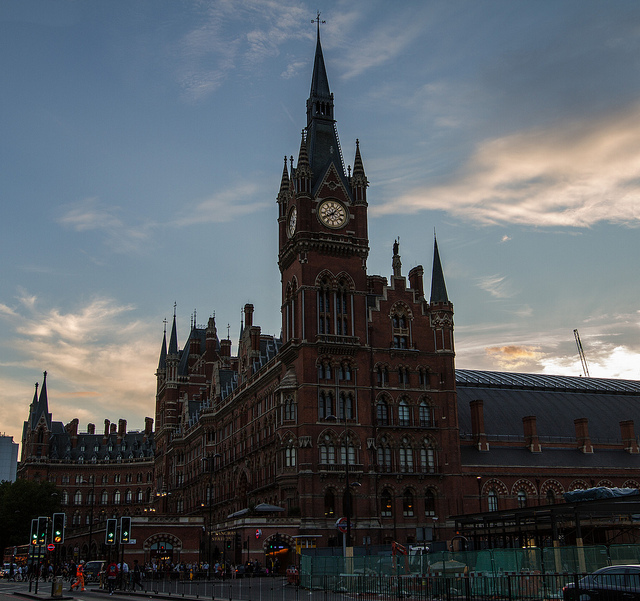
\includegraphics[width=0.7\linewidth]{imagens/st-pancreas.jpg}
     \label{fig:8}
     \footnote{\textbf{Fonte:} \cite{bromonschenkel2024cocopt}}
\end{figure}

A Tabela \ref{tab:3} apresenta as descrições geradas por cada modelo para a Figura \ref{fig:8}, bem como indicações resumidas da latência observada. A análise indica que o modelo \texttt{Qwen2.5-VL-7B-Instruct} foi capaz de capturar de forma mais precisa e contextualizada os elementos da imagem, identificando corretamente a estação e fornecendo detalhes arquitetônicos. Em contraste, o \texttt{llava-v1.6-mistral-7b-hf} não chega a nomear o edifício, ainda que descreva corretamente suas características gerais. Já o \texttt{Llama-3.2-11B-Vision-Instruct} apresentou alto tempo de processamento e resultados inferiores aos dois modelos, conforme já discutido na análise quantitativa.

\begin{table}[]
\centering
\caption{Comparação qualitativa das descrições geradas para a Figura \ref{fig:8}}
\label{tab:3}
\resizebox{\columnwidth}{!}{%
\begin{tabular}{@{}
>{\columncolor[HTML]{FFFFFF}}l 
>{\columncolor[HTML]{FFFFFF}}l 
>{\columncolor[HTML]{FFFFFF}}l @{}}
\toprule
\multicolumn{1}{c}{\cellcolor[HTML]{FFFFFF}\textbf{Modelo}} &
  \multicolumn{1}{c}{\cellcolor[HTML]{FFFFFF}\textbf{Descrição Gerada}} &
  \multicolumn{1}{c}{\cellcolor[HTML]{FFFFFF}\textbf{Latência (s)}} \\ \midrule
\texttt{llava-v1.6-mistral-7b-hf} &
  Você está vendo uma imagem de um grande edifício histórico, provavelmente uma torre de uma catedral ou igreja. A torre é alta e possui um relógio no topo, o que é comum em edifícios históricos. O edifício tem uma arquitetura ornamental e possui uma fachada rica em detalhes. O céu está parcialmente nublado, indicando que pode ser um dia com um pouco de nuvens. Ao fundo, há outros edifícios que parecem ser parte do complexo da catedral ou igreja. &
  7,0 \\
\texttt{Qwen2.5-VL-7B-Instruct} &
  Você está olhando para a St Pancras International Station, um edifício icônico localizado em Londres, Reino Unido. É reconhecível pela sua torre alta e elegante com um relógio no topo. A construção é feita de tijolos vermelhos e tem uma arquitetura gótica revivalista. À frente do edifício, há uma área aberta com algumas pessoas caminhando e veículos à distância. O céu está claro com algumas nuvens dispersas, sugerindo que é uma tarde tranquila. Não há riscos aparentes na imagem. &
  4,2 \\
\texttt{Llama-3.2-11B-Vision-Instruct} &
  Nesta imagem há uma grande construção com muitas janelas em diferentes níveis, possivelmente um prédio de apartamentos ou escritórios. A parte central da imagem contém três torres pontiagudas conectadas por uma estrutura que parece ser uma passagem ou uma galeria. Há também uma grande relógio na torre do meio.  A construção está coberta em sua maioria com tijolos vermelhos, mas há alguns detalhes decorativos de pedra nas janelas e nos cantos das torres. Há um pequeno pátio ou espaço aberto ao lado da construção, possivelmente uma área de descanso ou um local de encontro.  A imagem é capturada em silhueta contra o céu escuro, o que sugere que a foto foi tirada durante o entardecer ou à noite. A luz solar não está diretamente na câmera, mas há algumas sombras claras nas áreas mais escuras da construção e do pátio.  É uma imagem clássica de uma estrutura histórica, possivelmente um edifício de importância cultural ou um marco arquitetônico. &
  56,5 \\ \bottomrule
\end{tabular}%
}
\end{table}

Já na Figura 9, temos a fotografia de uma garrafa de água posicionada sobre uma mesa em um ambiente interno, com iluminação artificial e diversos objetos ao redor (discos, controles remotos, documentos). Esse cenário foi escolhido para avaliar a capacidade dos modelos em identificar elementos cotidianos e ambientes com luminosidade reduzida.

\begin{figure}[!ht]
     \caption{Fotografia de uma garrafa sobre uma mesa com objetos}
     \centering
     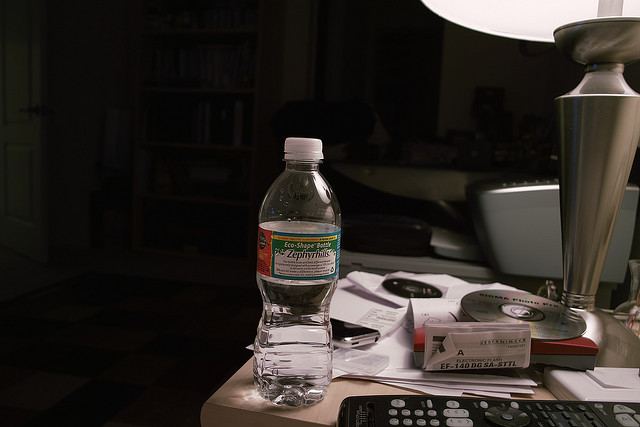
\includegraphics[width=0.7\linewidth]{imagens/garrafa.jpg}
     \label{fig:9}
     \footnote{\textbf{Fonte:} \cite{bromonschenkel2024cocopt}}
\end{figure}

A Tabela \ref{tab:4} ilustra as descrições geradas pelos modelos para a Figura \ref{fig:9}. Observa-se novamente que o \texttt{Qwen2.5-VL-7B-Instruct} apresenta uma descrição mais detalhada, mencionando itens como “luminária de mesa com abajur branco” e “discos compactos”. Já o \texttt{llava-v1.6-mistral-7b-hf} acerta em vários pontos, mas inclui elementos que não são claramente visíveis (ou que descreve de forma menos precisa) e mantém maior latência. Quanto ao \texttt{Llama-3.2-11B-Vision-Instruct}, os problemas de infraestrutura e latência novamente prejudicaram a viabilidade de uso no protótipo.

\begin{table}[]
\centering
\caption{Comparação qualitativa das descrições geradas para a Figura \ref{fig:9}}
\label{tab:4}
\resizebox{\textwidth}{!}{%
\begin{tabular}{@{}
>{\columncolor[HTML]{FFFFFF}}l 
>{\columncolor[HTML]{FFFFFF}}l 
>{\columncolor[HTML]{FFFFFF}}l @{}}
\toprule
\multicolumn{1}{c}{\cellcolor[HTML]{FFFFFF}{\color[HTML]{000000} \textbf{Modelo}}} &
  \multicolumn{1}{c}{\cellcolor[HTML]{FFFFFF}{\color[HTML]{000000} \textbf{Descrição Gerada}}} &
  \multicolumn{1}{c}{\cellcolor[HTML]{FFFFFF}{\color[HTML]{000000} \textbf{Latência (s)}}} \\ \midrule
{\color[HTML]{000000} \texttt{llava-v1.6-mistral-7b-hf}} &
  {\color[HTML]{000000} Você está vendo uma imagem de uma lâmpada de escritório com um garfo de luz aceso, um botão de mando e um controle remoto. A lâmpada está em um ambiente escuro, com uma mesa de escritório ao fundo, onde há livros e outros itens. No centro da imagem, há uma garrafa de água com uma etiqueta que diz "Fruit Shape Zephyr". A garrafa está em um ambiente que parece ser um escritório ou uma área de trabalho.} &
  {\color[HTML]{000000} 5,5} \\
{\color[HTML]{000000} \texttt{Qwen2.5-VL-7B-Instruct}} &
  {\color[HTML]{000000} Na imagem, há uma garrafa de água mineral em destaque no centro, posicionada sobre uma superfície que parece ser uma mesa ou um suporte de papel. Ao fundo, há uma luminária de mesa com um abajur branco e uma base metálica. À direita da garrafa, há alguns discos compactos (CDs) empilhados sobre um pacote de papel. Embaixo da garrafa, há alguns documentos e um controle remoto. O ambiente parece ser um escritório ou sala de estar, com uma porta fechada à esquerda e prateleiras com livros ao fundo. A iluminação é baixa, sugerindo que a foto foi tirada à noite ou em um local escuro. Não há riscos aparentes na imagem.} &
  {\color[HTML]{000000} 5,2} \\
{\color[HTML]{000000} \texttt{Llama-3.2-11B-Vision-Instruct}} &
  {\color[HTML]{000000} A imagem mostra uma mesa com alguns objetos sobre ela. Há uma garrafa de água, provavelmente de 1 litro, na parte central da imagem. À direita dela está um CD, que parece estar sobre um livro ou outro objeto. No fundo, há a silhueta de um computador. A luz do monitor cria uma sombra no lado esquerdo da mesa e acaba de cima do CD.} &
  {\color[HTML]{000000} 22,5} \\ \bottomrule
\end{tabular}%
}
\end{table}

Desta forma, com base nos resultados quantitativos e qualitativos, fica claro que o \texttt{Qwen2.5-VL-7B-Instruct} desponta como o modelo mais adequado para a integração no protótipo assistivo, sobretudo pela sua latência significativamente menor. Embora o modelo \texttt{Llama-3.2-11B-Vision-Instruct} apresente uma boa qualidade textual, mesmo removendo ou adicionando informações não presentes nas imagens, as limitações de infraestrutura e os altos tempos de resposta comprometem sua aplicabilidade, mesmo quando integrado por meio do Ollama. Da mesma forma, embora o \texttt{llava-v1.6-mistral-7b-hf} seja uma opção viável, sua performance em latência é inferior à do \texttt{Qwen}, fator decisivo para aplicações em tempo real.

Esses resultados indicam que, para o desenvolvimento do protótipo assistivo, a priorização do desempenho em termos de latência, além da qualidade textual, é fundamental. Assim, o \texttt{Qwen2.5-VL-7B-Instruct} desponta como o modelo preferencial, oferecendo um compromisso entre qualidade textual, detalhamento contextual e velocidade de processamento, o que se confirma tanto nos testes quantitativos quanto na comparação qualitativa das descrições geradas.

\section{Testes da Aplicação}

Após a conclusão do \textit{benchmark} e a consequente escolha do \texttt{Qwen2.5-VL-7B-Instruct} como modelo mais adequado, procedeu-se à avaliação prática do protótipo completo, composto pelo aplicativo em Flutter, a API em Python (usando FastAPI) e o referido modelo de IA. Embora também tenham sido realizadas breves avaliações com os outros dois modelos (\texttt{llava-v1.6-mistral-7b-hf} e \texttt{Llama-3.2-11B-Vision-Instruct}) para confirmar as conclusões do \textit{benchmark}, as análises mais aprofundadas concentraram-se no \texttt{Qwen2.5-VL-7B-Instruct}, uma vez que sua menor latência e melhor qualidade de descrição se mostraram determinantes para a experiência de uso pretendida.

Os testes realizados entre os três modelos evidenciaram que o \texttt{Qwen2.5-VL-7B-Instruct} efetivamente se mantém como a opção mais apropriada para a solução proposta. Observou-se, na prática, o mesmo padrão identificado na seção anterior: o modelo oferece um tempo de resposta significativamente menor, fator crucial para aplicações assistivas, e produz descrições mais consistentes, com menor propensão a “alucinações” ou erros semânticos. Esse equilíbrio entre desempenho e clareza textual consolida o \texttt{Qwen2.5-VL-7B-Instruct} como a alternativa mais confiável e eficiente para o desenvolvimento do protótipo.

\subsection{Avaliação Prática do Protótipo}

Tendo definido o \texttt{Qwen2.5-VL-7B-Instruct} como o modelo mais apropriado, procedeu-se a testes práticos para validar o funcionamento integrado do aplicativo em Flutter, da API em Python (via FastAPI) e do próprio modelo de IA. O objetivo principal foi verificar se o protótipo realmente atende às necessidades de pessoas com deficiência visual, tanto em termos de acessibilidade de interface quanto de coerência das descrições fornecidas.

\subsubsection{Estrutura e Fluxo de Interação}

O aplicativo em Flutter foi concebido com uma interface minimalista, a fim de tornar o uso mais simples para quem depende de recursos de acessibilidade. Logo ao iniciar, o TTS reproduz uma mensagem de boas-vindas, instruindo o usuário: basta tocar na tela para iniciar a gravação de áudio e a captura da imagem, e tocar novamente para encerrar o processo, enviando a solicitação para processamento e aguardando a resposta. Dessa forma, reduz-se a dependência de diversos botões ou elementos visuais, conferindo à aplicação uma usabilidade mais direta e inclusiva.

Na Figura \ref{fig:10} pode-se ver a tela inicial do aplicativo, que evidencia a interface minimalista, sendo a tela toda basicamente a imagem da câmera do dispositivo. É apresentado na Figura \ref{fig:11}, o momento que o usuário realiza o primeiro toque na tela, iniciando o processo de captura da imagem e também de gravação do áudio, que é finalizado pelo segundo toque na tela, resultando na Figura \ref{fig:12}. Na sequência, a imagem e o áudio são enviados à API, que faz uso do \texttt{Qwen2.5-VL-7B-Instruct} para gerar uma descrição da imagem que foi capturada. Em seguida, o aplicativo reproduz automaticamente a descrição retornada, completando o ciclo de interação sem a necessidade de múltiplas interfaces ou botões.

\begin{figure}[!ht]
     \caption{Tela inicial do aplicativo}
     \centering
     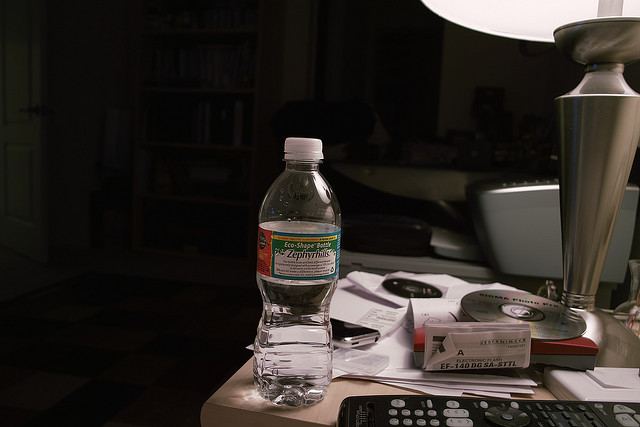
\includegraphics[width=0.7\linewidth]{imagens/garrafa.jpg}
     \label{fig:10}
     \footnote{\textbf{Fonte:} Elaborado pelo Autor (2025)}
\end{figure}

\begin{figure}[!ht]
     \caption{Tela após o início da gravação e captura da imagem}
     \centering
     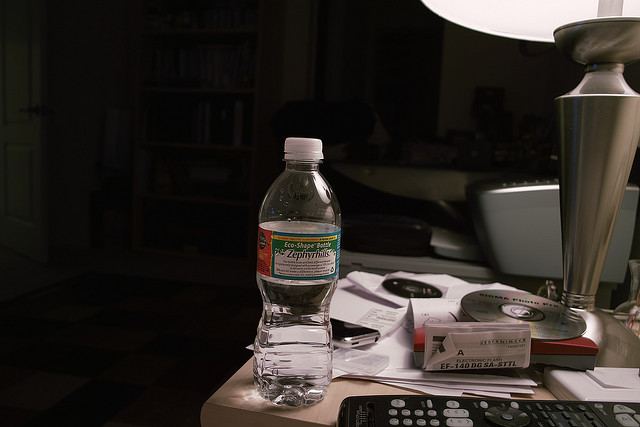
\includegraphics[width=0.7\linewidth]{imagens/garrafa.jpg}
     \label{fig:11}
     \footnote{\textbf{Fonte:} Elaborado pelo Autor (2025)}
\end{figure}

\begin{figure}[!ht]
     \caption{Tela após o segundo toque e envio da solicitação à API}
     \centering
     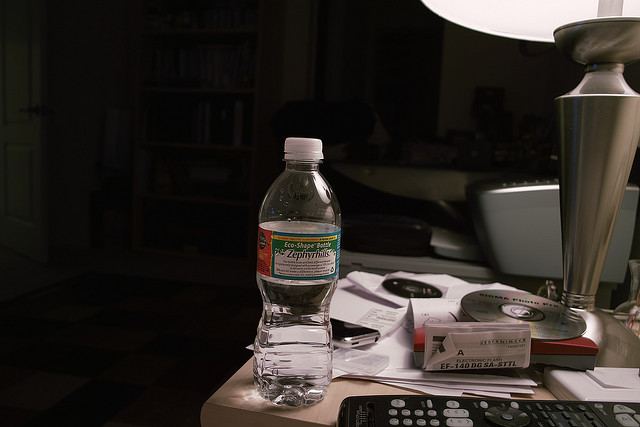
\includegraphics[width=0.7\linewidth]{imagens/garrafa.jpg}
     \label{fig:12}
     \footnote{\textbf{Fonte:} Elaborado pelo Autor (2025)}
\end{figure}

\subsubsection{Desempenho e Qualidade das Descrições}

Os testes realizados em diversos cenários — ambientes internos com baixa iluminação, áreas externas sob luz natural intensa, presença de múltiplos objetos — corroboraram a eficiência do \texttt{Qwen2.5-VL-7B-Instruct} apontada no \textit{benchmark}. Em termos de desempenho, constatou-se que o tempo entre a captura da imagem e a transmissão do áudio final ao usuário permaneceu baixo, viabilizando a sensação de tempo real. Esse resultado decorre, em grande parte, da menor latência do modelo escolhido em comparação com os demais modelos avaliados.

Quanto à qualidade das descrições, observou-se que o \texttt{Qwen2.5-VL-7B-Instruct} geralmente forneceu legendas coerentes e detalhadas. Mesmo em situações mais complexas, a identificação dos elementos principais se manteve satisfatória, embora algumas descrições possam omitir detalhes ou interpretar incorretamente alguns objetos e situações presentes na imagem. Na maioria dos testes, porém, o conteúdo foi suficiente para dar ao usuário uma noção clara do ambiente, alinhando-se ao objetivo assistivo proposto.

Pode-se avaliar o resultado final tomando como exemplo a imagem retirada da Figura 10, onde foi realizado o processo inicial da captura da imagem e gravação do áudio, conforme evidenciam as Figuras \ref{fig:11} e \ref{fig:12}. Neste caso, ao ser enviada a solicitação à API, o modelo realizou a inferência e retornou a seguinte resposta: "Lorem ipsum dolor sit amet, consectetur adipiscing elit, sed do eiusmod tempor incididunt ut labore et dolore magna aliqua. Ut enim ad minim veniam, quis nostrud exercitation ullamco laboris nisi ut aliquip ex ea commodo consequat. Duis aute irure dolor in reprehenderit in voluptate velit esse cillum dolore eu fugiat nulla pariatur. Excepteur sint occaecat cupidatat non proident, sunt in culpa qui officia deserunt mollit anim id est laborum."

\subsubsection{Acessibilidade e Integração}

A utilização contínua do TTS durante todo o ciclo de uso garante que o sistema seja efetivamente acessível, possibilitando que o usuário receba instruções e descrições em áudio sem a necessidade de auxílio visual ou suporte adicional. Paralelamente, a API abstrai a complexidade do modelo de IA, de modo que o aplicativo em Flutter se mantém leve e simples de operar em qualquer dispositivo móvel compatível.

Com esse design modular, a robustez do servidor e do modelo, incluindo possíveis evoluções ou substituições futuras, não altera a experiência de quem utiliza o aplicativo. Isso potencializa a escalabilidade e a flexibilidade do sistema, contribuindo para que a solução possa ser continuamente atualizada sem comprometer o foco assistivo.

\subsubsection{Síntese dos Resultados}

A avaliação prática do sistema revelou três aspectos fundamentais para o sucesso da proposta. Em primeiro lugar, a baixa latência efetiva proporcionou respostas ágeis, fator indispensável em aplicações assistivas que demandam \textit{feedback} quase imediato. Em segundo lugar, as descrições fornecidas pelo \texttt{Qwen2.5-VL-7B-Instruct} mostraram-se suficientemente coerentes para oferecer ao usuário uma compreensão geral do ambiente, cumprindo com êxito o papel de fornecer legendas informativas na maioria dos cenários testados.

Por fim, a integração do TTS ao longo de todo o fluxo de interação evidenciou o potencial inclusivo do protótipo, tornando o sistema acessível e viabilizando a utilização independente por pessoas com deficiência visual. Assim, conclui-se que o protótipo não apenas se apoia em um modelo de IA robusto, mas também adota uma interface voltada ao público-alvo, garantindo praticidade, rapidez e uma experiência de uso imersiva.

\section{Análise Crítica dos Resultados}

A avaliação prática do protótipo integrado — aplicativo Flutter, API em Python e modelo \texttt{Qwen2.5-VL-7B-Instruct} — evidenciou que a escolha do modelo se revelou eficaz tanto no quesito latência quanto na qualidade das descrições. A baixa latência possibilitou que o usuário recebesse as informações de modo quase imediato, fator imprescindível para aplicações assistivas. Nesse sentido, o \texttt{Qwen2.5} provou ser uma opção mais equilibrada do que os demais modelos testados, que enfrentaram problemas de alto consumo de memória ou tempos de resposta excessivos.

Do ponto de vista do TTS, a experiência de uso foi satisfatória. A adoção de mensagens de áudio em cada etapa reduziu a dependência de interfaces visuais, assegurando que o protótipo estivesse plenamente alinhado aos princípios de acessibilidade. Ainda assim, é importante salientar que a precisão das descrições pode variar em cenários de maior complexidade visual, ou quando a iluminação é precária. Nessas situações, o modelo pode apresentar falhas pontuais de identificação ou omissões. Não obstante, no conjunto das avaliações, o sistema cumpriu seu objetivo de prover ao usuário uma visão geral do ambiente, demonstrando o potencial de integração entre tecnologias de visão computacional, modelos de linguagem e aplicações mobile para promover inclusão digital.

O projeto também revela um \textit{trade-off} claro entre desempenho e robustez. Embora o \texttt{Qwen2.5} ofereça respostas confiáveis em tempo razoável, modelos maiores (como o \texttt{Llama-3.2-11B-Vision-Instruct}) poderiam, em teoria, gerar descrições mais ricas, porém à custa de maior latência e requisitos de \textit{hardware}. A escolha final recai, pois, sobre a necessidade de um equilíbrio entre esses fatores, priorizando a experiência do usuário com deficiência visual, que requer fluidez e respostas rápidas para contextos do cotidiano.

\section{Limitações}

Apesar dos resultados promissores, o trabalho apresenta algumas limitações que precisam ser consideradas. Em primeiro lugar, há a dependência de uma conexão com a internet para que o protótipo possa se comunicar com o servidor remoto, onde está hospedado o modelo de IA. Em regiões com acesso precário ou instável à rede, essa característica tende a aumentar a latência ou até mesmo inviabilizar o funcionamento do sistema. Além disso, a execução de testes com centenas de imagens revelou que a capacidade de GPU disponível foi ocasionalmente excedida, evidenciando a necessidade de recursos computacionais mais robustos ou de técnicas mais avançadas de otimização, como a quantização mais avançada ou distribuição de carga em múltiplas instâncias de servidores, para garantir um desempenho consistente em larga escala.

Outro ponto a destacar diz respeito ao comportamento do modelo em cenários de alta complexidade visual. Embora o modelo definido ofereça descrições satisfatórias na maioria das situações, imagens muito sobrecarregadas de detalhes ou mal iluminadas podem resultar em legendas incompletas ou confusas, exigindo técnicas adicionais de pré-processamento de imagens ou modelos especializados em tais condições. Também vale ressaltar que, apesar de os testes internos terem indicado uma boa experiência, não foram realizadas avaliações extensivas com um público diversificado de pessoas com deficiência visual, de modo que a validação do protótipo em cenários reais de mobilidade e diferentes perfis de usuários permanece como uma lacuna a ser suprida em trabalhos futuros.

Por fim, é importante considerar que o sistema desenvolvido se configura como um protótipo experimental, cujo foco principal foi demonstrar a viabilidade de integrar um modelo de IA relativamente robusto em um aplicativo destinado à acessibilidade. Assim, essas limitações não anulam o mérito dos resultados obtidos, mas apontam caminhos concretos para avanços, seja no aprimoramento da infraestrutura de processamento, seja na incorporação de técnicas adicionais de otimização e na ampliação dos testes de campo com usuários finais.


\chapter{Conclusões} \label{cap:05}

A implementação de um aplicativo capaz de descrever o ambiente e apresentar as informações por meio de áudio para pessoas com deficiência visual teve, como ponto-chave, a comparação de diferentes LLMs. Essa comparação foi essencial para determinar o equilíbrio adequado entre qualidade das descrições e desempenho em tempo real, culminando na escolha do \texttt{Qwen2.5-VL-7B-Instruct} como a alternativa mais viável. Ao longo do trabalho, constatou-se que a menor latência e a robustez na geração de descrições deste modelo se destacaram em relação às demais opções avaliadas, contribuindo diretamente para uma experiência de uso mais fluida.

Os resultados obtidos demonstram que os objetivos foram alcançados: o desenvolvimento de um protótipo funcional, acessível e capaz de auxiliar usuários com deficiência visual na percepção do mundo ao redor. A utilização de LLMs \textit{open source} reforça a relevância social e tecnológica da solução, pois permite a evolução contínua do projeto com base em avanços na comunidade de pesquisa e desenvolvimento. Além disso, a adoção de uma arquitetura modular, na qual o aplicativo móvel e a API de processamento são facilmente intercambiáveis, reforça a flexibilidade do sistema, mostrando que modelos multimodais e avançados podem ser integrados de maneira relativamente simples.

Para trabalhos futuros, algumas direções podem levar a ganhos significativos de desempenho e acessibilidade. Em primeiro lugar, a execução direta dos modelos de LLM no dispositivo móvel, reduzindo ou eliminando a necessidade de conexão à internet, representa um passo importante para usuários em regiões de acesso limitado. Associada a isso, a aplicação de técnicas mais avançadas de otimização, seja pela redução de parâmetros ou pelo desenvolvimento de arquiteturas mais enxutas, pode diminuir a latência e os custos de execução. Também se vislumbra a possibilidade de aprimorar o TTS, tornando-o mais natural, e de estender a robustez do sistema, de modo que ele mantenha qualidade em diferentes condições ambientais, tais como iluminação adversa ou ambientes muito complexos. Dessa forma, o protótipo abre caminho para novas pesquisas e aprimoramentos, reforçando o papel das tecnologias assistivas no fortalecimento da inclusão digital.
% \chapter{Cronograma}  \label{cap:07}

% Esse capítulo só se insere na Versão da Pré Banca. Na Versão da Defesa ele é retirado já que o cronograma deverá ter sido concluído.

\begin{table}[!h]
\begin{tabular}{|c|c|c|c|c|c|c|c|c|c|c|}
\hline
\multirow{2}{*}{\textbf{Descrição das Atividades}} & \multicolumn{10}{c|}{\textbf{Meses}}            \\ \cline{2-11} 
                                                   & 01 & 02 & 03 & 04 & 05 & 06 & 07 & 08 & 09 & 10 \\ \hline
Atividade 1                                        &    & $\bullet$ & $\bullet$  &    &    &    &    &    &    &    \\ \hline
Atividade 2                                        &    &    & $\bullet$  & $\bullet$  &    &    &    &    &    &    \\ \hline
Atividade 3                                        &    &    &    & $\bullet$  &    &    &    &    &    &    \\ \hline
Atividade 4                                        &    &    &    &    &    &    &    &    &    &    \\ \hline
Atividade 5                                        &    &    &    &    &    &    &    &    &    &    \\ \hline
Atividade 6                                        &    &    &    &    &    &    &    &    &    &    \\ \hline
\end{tabular}
\end{table}


No cronograma você irá inserir as atividades que irá realizar, bem como marcar com a bolinha nos meses que irá realizá-las. Como estamos no Latex, a edição dessas tabelas deve ser realizada em um programa que trabalhe com configuração de tabelas.
Para isso, você deve seguir os seguintes passos:

\begin{enumerate}
    \item Copie o código da tabela acima.
    \item Acesse o seguinte site: \href{https://www.tablesgenerator.com/latex_tables#}{Editor de Tabelas} ;
    \item Clique em "File";
    \item Clique em "From Latex Code";
    \item Cole o Texto da tabela copiada e clique em "Load";
\end{enumerate}

Esse procedimento irá gerar uma tabela como a que está acima. Basta editar conforme sua necessidade, alterando as atividades e o nome dos meses e posicionando a bolinha nos quadrados dos meses em que as atividades serão realizadas.

Posteriormente basta clicar em "Generate", copiar o código e substituir a tabela acima por ele.

% ----------------------------------------------
%         Referências bibliográficas
% ----------------------------------------------

%\bibliographystyle{plain}
\bibliography{referencias.bib}

% ----------------------------------------------
%            ELEMENTOS PÓS-TEXTUAIS
% ----------------------------------------------
%\postextual

% -----------------------------------------------
%                  Glossário
% -----------------------------------------------
%
% Consulte o manual da classe abntex2 para orientações sobre o glossário.
%%\glossary

% ------------------------------------------------
% Apêndices
% ------------------------------------------------
%% Texto ou documento elaborado pelo autor, a fim de complementar sua argumentação, sem prejuízo da unidade nuclear do trabalho.

% ---
% Inicia os apêndices
% ---
\begin{apendicesenv}
	
	% Imprime uma página indicando o início dos apêndices
	%\partapendices
	
	% ----------------------------------------------------------
	\chapter{Título do Apêndice A}
	% ----------------------------------------------------------
	
	Texto do Apêndice A.
	
	.
		
	
\end{apendicesenv}
% ---
% ----------------------------------------------------------
% Anexos
% ----------------------------------------------------------
%% Texto ou documento não elaborado pelo autor, que serve de fundamentação, comprovação e/ou ilustração.

% ---
% Iniciam os anexos
% ---
\begin{anexosenv}
	
	% Imprime uma página indicando o início dos anexos
	% \partanexos
	
	% ----------------------------------------------------------
	\chapter{Título do Anexo A}
	% ----------------------------------------------------------
	
	Texto do Anexo A.
	
	
\end{anexosenv}
%-----------------------------------------------------------
% ÍNDICE REMISSIVO
%-----------------------------------------------------------

%\phantompart

% \printindex

\end{document}
